%!TEX root = colt2018.tex
 
\clearpage

{\LARGE Organization of the Appendix}

\vspace{0.25cm}

\begin{enumerate}

\item[\ref{ap:experiments}.] {\em Experiments} \\where the experiments and their settings are explained.

\item[\ref{sec:proba}.] {\em Probabilistic lemmas} \\where concentration inequalities in Hilbert spaces used in section \ref{sec:AppSGD} are recalled.

\item[\ref{sect:proof-A5-to-01}.] {\em From $\H$ to 0-1 loss} \\where, from high probability bound for $\|\cdot\|_\H$, we derived bound for the 0-1 error.

\item[\ref{sect:exp-rates-for-KRR}.] {\em Proofs of Exponential rates for Kernel Ridge Regression} \\where exponential rates for Kernel Ridge Regression are proven (Theorem \ref{thm:exp-class-krls}).

\item[\ref{sect:examples-for-glambda}.] {\em Proofs and additional results about concrete examples} \\where additional results and croncrete examples to satisfy \asm{asm:flambda-correct-sign} are given.

\item[\ref{ap:SGDdevelopment}.] {\em Preliminaries for Stochastic Gradient Descent} \\where the SGD recursion is derived.

\item[\ref{sec:AppSGD}.] {\em Proof of stochastic gradient descent results} \\ where high probability bounds for the general SGD recursion are shown (Theorems \ref{th:SGDalpha} and \ref{th:SGDaveraged}).

\item[ \ref{sec:error}.] {\em Exponentially convergent SGD for classification error} \\where exponential convergence of test error are shown (Theorems \ref{th:erroralpha} and \ref{th:errortail}).

\item[\ref{ap:average}.] {\em Extension for the full averaged case} \\where previous results are extended for full averaged SGD (instead of tail-averaged).

\item[\ref{ap:weakmargin}.] {\em Convergence under weaker margin assumption} \\where previous results are extended in the case of a weaker margin assumption.
\end{enumerate}

\section{Experiments} \label{ap:experiments}

To illustrate our results, we consider one-dimensional synthetic examples ($\X = [0,1] $) for which our assumptions are easily satisfied. 
Indeed, we consider the following set-up that fulfils our assumptions: 
\BIT
\item \asm{asm:separability}, \asm{asm:data-iid} We consider here $X \sim U\left([0,(1-\varepsilon)/2] \cup [(1+\varepsilon)/2,1]  \right)$ and with the notations of Example \ref{ex:independent-noise-on-labels}, we take $\mathcal{S}_+ = [0,(1-\varepsilon)/2]$ and $\mathcal{S}_- = [(1+\varepsilon)/2,1]$. For $1 \leq i \leq n$,  $x_i$ independently sampled from $\rhox$ we define $y_i = 1 $ if $x_i \in \mathcal{S}_+$ and $y_i = -1 $ if $x_i \in \mathcal{S}_-$.

\item \asm{asm:kernel-bounded} We take the kernel to be the exponential  kernel $K(x,x') = \exp(-|x-x'|)$ for which the RKHS is a Sobolev space $\H = W^{s,2}$, with $s > d/2$, which is dense in $L_2$~\citep{adams2003sobolev}.

\item \asm{asm:flambda-correct-sign} With this setting we could find a closed form for $g_\lambda$ and checked that it verified \asm{asm:flambda-correct-sign}. Indeed we could solve the optimality equation satisfied by $g_\lambda$ : $$ \forall z \in [0,1], \ \int_{0}^1 K(x,z)g_\lambda(x) d\rho_X(x) + \lambda g_\lambda(z) = \int_{0}^1 K(x,z)g_\rho(x) d\rho_X(x),  $$ the solution being a linear combination of exponentials in each set : $[0,(1-\varepsilon)/2]$, $[(1-\varepsilon)/2,(1+\varepsilon)/2]$ and $[(1+\varepsilon)/2,1]$.
\EIT

\begin{figure}[ht]
    \centering
    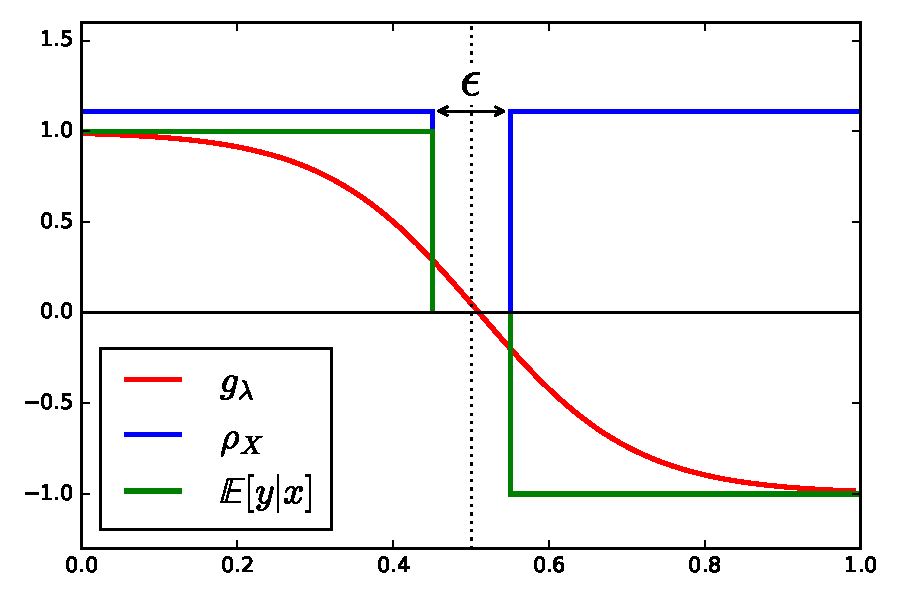
\includegraphics[width=0.45\textwidth]{figures/zbis_densities.pdf}
    \caption{Representing the $\rho_\X$ density (uniform with $\varepsilon$-margin), the best estimator, i.e., $\E (x|y)$ and $g_\lambda$ used for the simulations ($\lambda = 0.01$).}
    \label{fig:densities}
\end{figure}

%
In the case of SGD with decreasing step size, we computed only the test error $\mathbb{E}({\cal R}(g_n)-{\cal R}^*))$. For tail averaged SGD with constant step size, we computed the test error as well as the training error, the test loss (which corresponds to the $L_2$ loss : $\int_0^1 (g_n (x) - g_\lambda(x))^2d\rho(x)$) and the training loss.
%
In all cases we computed the errors of the $n$-th iterate with respect to the calculated $g_\lambda$, taking $g_0 = 0$. For any $n \geqslant 1$,
$$g_n  =  {g}_{n-1} - \gamma_n  \big[ ( {g}_{n-1}(x_n)- y_n)K_{x_n}   + \lambda{g}_{n-1}  \big]. $$

We can use representants to find the recursion on the coefficients. Indeed, if  $g_n = \sum_{i = 1}^n a^n_i K_{x_i},$ then the following recursion for the $(a_i^n)$ reads : 
\begin{eqnarray*}
\text{for } i \leqslant n-1, \ a_i^n &=& (1-\gamma_n \lambda) a_i^{n-1} \\
a_n^n &=& -\gamma_n (\sum_{i = 1}^{n-1} a_i^{n-1} K(x_n,x_i)-y_n).
\end{eqnarray*}
%
From $(a_i^n)$, we can also compute the coefficients of $\bar{g}_n$ and $\bar{g}_n^{\textrm {tail}}$ that we note $\bar{a}^n_i$ and $\bar{a}^{n,\textrm {tail}}_i$ respectively: $\bar{a}^n_i = \sum_{k = i}^n \frac{a_i^k}{n+1}$ and $\bar{a}^{n,\textrm {tail}}_i = \frac{1}{\lfloor n/2 \rfloor}\sum_{k = \lfloor n/2 \rfloor }^n a_i^k.$
%
To show our theoretical results we have decided to present the following figures: 

\BIT
\item For the exponential convergence of the averaged and tail averaged cases, we plotted the error $\log_{10}\mathbb{E}({\cal R}(g_n)-{\cal R}^*))$ as a function of $n$. With this scale and following our results it goes as a line after a certain $n$ (Figures \ref{fig:plots} and \ref{fig:techplots} right).
\item We recover the results of \citet{daft} that show convergence at speed $1/n$ for the loss (Figure \ref{fig:plots} left). We adapted the scale to compare with the error plot.
\item For Figure \ref{fig:techplots} left, we plotted $-\log (- \log (\mathbb{E}({\cal R}(g_n)-{\cal R}^*)) ) $ of the excess error with respect to the $\log$ of $n$ to show a line of slope $-1/2$. It meets our theoretical bound of the form $\exp(-K\sqrt{n})$, 
\EIT

Note that for the plots where we plotted the expected excess errors, i.e., $\mathbb{E}({\cal R}(g_n)-{\cal R}^*)$, we plotted the mean of the errors over 1000 replications until $n = 200$, whereas for the plots where we plotted the losses, i.e., a function of $\|g_n- g_*\|_2$, we plotted the mean of the loss over 100 replications until $n = 2000$.

\begin{figure}[ht]
\footnotesize
\stackunder[1pt]{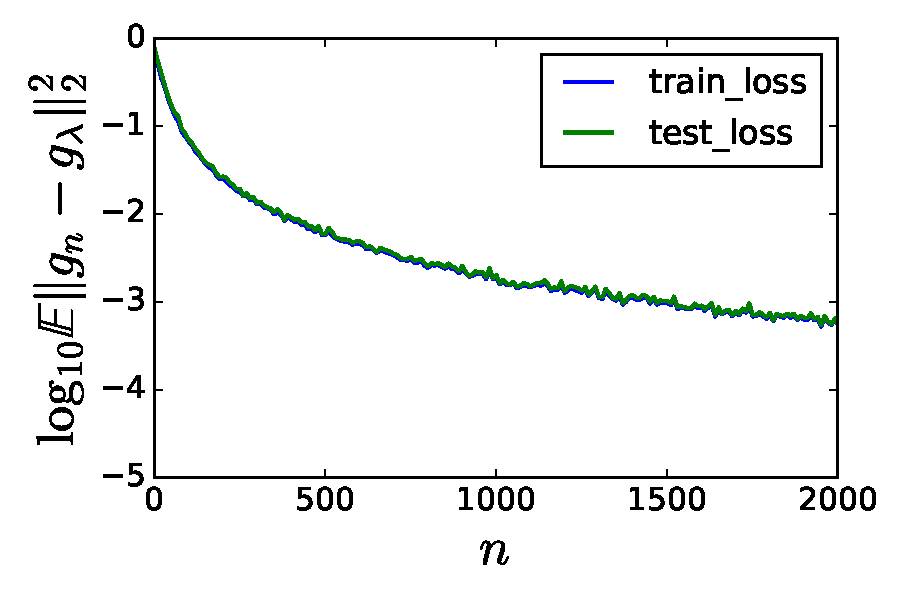
\includegraphics[width=0.48\textwidth]{figures/zbis_a_loss.pdf}}{}%
\hspace{1cm}%
\stackunder[1pt]{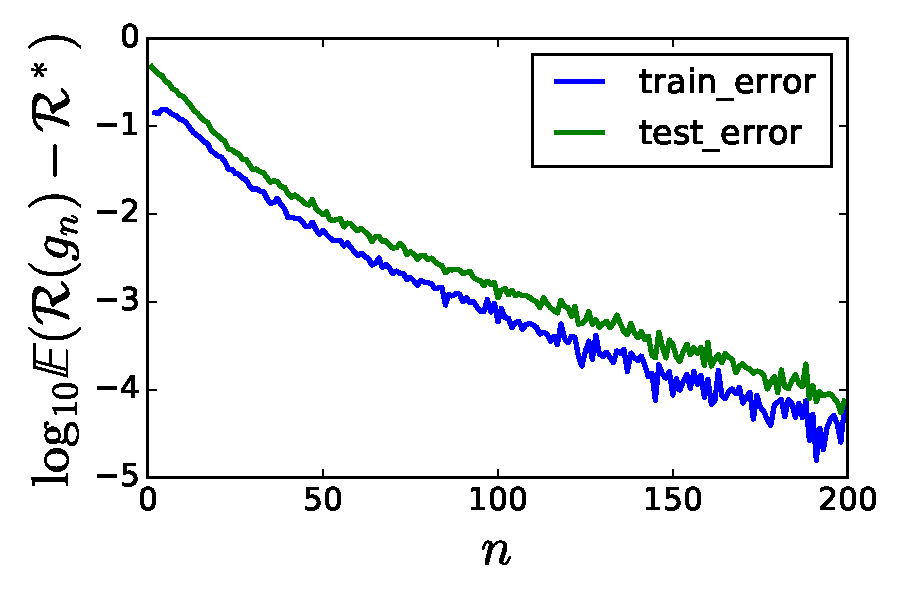
\includegraphics[width=0.48\textwidth]{figures/zbis_a_error.pdf}}{}%
\vspace{-0.5cm}
\caption{ \small Showing linear convergence for the $L^{01}$ errors in the case of margin of width $\varepsilon$. {\bfseries Left} figure corresponds to the test and training loss in the averaged case whereas the {\bfseries right} one corresponds to the error in the same setting. Note that the y-axis is the same while the x-axis is different of a factor 10. The fact that the error plot is a line after a certain $n$ matches our theoretical results. We took the following parameters :  $\varepsilon = 0.05$, $\gamma = 0.25$, $\lambda = 0.01$.}
\label{fig:plots}
\end{figure}
%
We can make the following observations:

First remark that between plots of losses and errors (Figure \ref{fig:plots} left and right resp.), there is a factor~10 between the numbers of samples (200 for errors and 2000 for losses) and another factor~10 between errors and losses ($10^{-4}$ for errors and $10^{-3}$ for losses). That underlines well our theoretical result which is the difference between exponential rates of convergence of the excess error and $1/n$ rate of convergence of the loss.

\begin{figure}[ht]
\footnotesize
\stackunder[1pt]{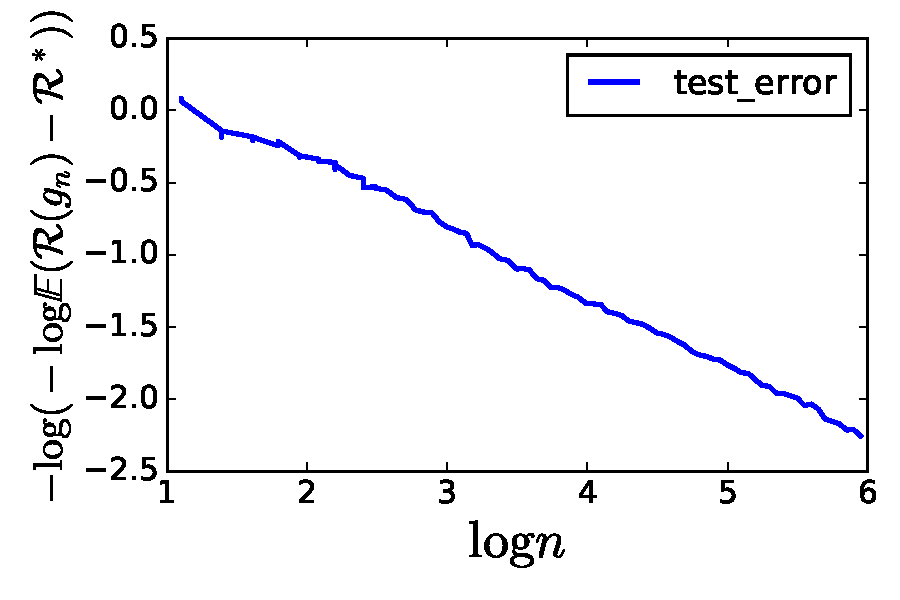
\includegraphics[width=0.48\textwidth]{figures/zbis_error_alpha.pdf}}{}%
\hspace{1cm}%
\stackunder[1pt]{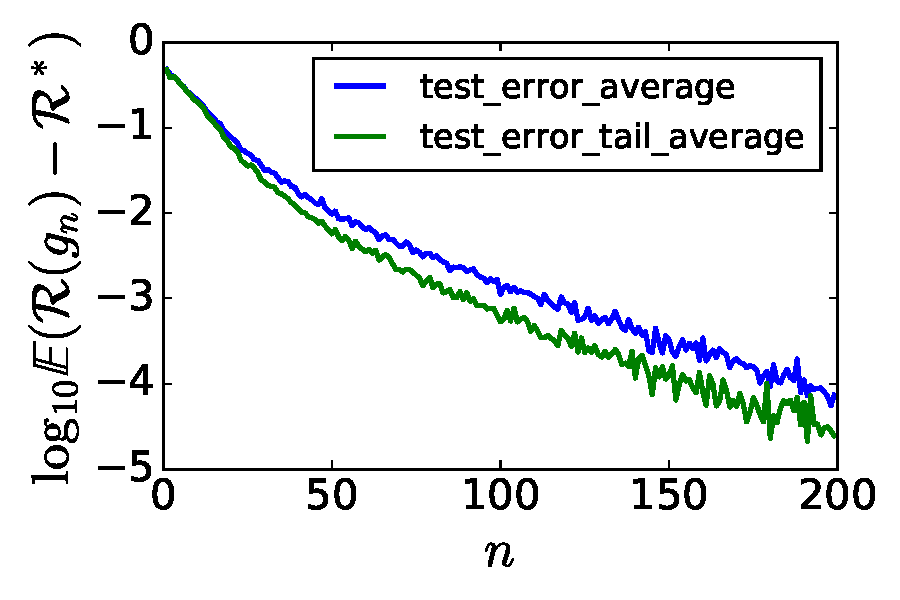
\includegraphics[width=0.48\textwidth]{figures/zbis_error_comparison.pdf}}{}
\vspace{-0.8cm}
\caption{ \small {\bfseries Left} plot shows the error in the non-averaged case for $\gamma_n = \gamma / \sqrt{n}$ and {\bfseries right} compares the test error between averaged and tail averaged case. We took the following parameters :  $\varepsilon = 0.05$, $\gamma = 0.25$, $\lambda = 0.01$.}
\label{fig:techplots}
\end{figure}

Moreover, we see that even if the excess error with tail averaging seems a bit faster, we have linear rates too for the convergence of the excess error in the averaged case. Finally, we remark that the error on the train set is always below the one for a unknown test set (of what seems to be close to a factor 2).





 \section{Probabilistic lemmas} \label{sec:proba}

In this section we recall two fundamental results for concentration inequalities in Hilbert spaces shown in \citet{pinelis1994optimum}.

\begin{proposition}
\label{Probabilisticprop}
Let $(X_k)_{k \in \mathbb{N}}$ be a sequence of vectors of $\mathcal{H}$ adapted to a non decreasing sequence of $\sigma$-fields $(\mathcal{F}_k)$ such that $\E \left[ X_k | \mathcal{F}_{k-1} \right] = 0$, $\sup_{k \leqslant n} \| X_k \| \leqslant a_n$ and $\sum_{k = 1}^n \E \left[ \|X_k\|^2 | \mathcal{F}_{k-1} \right] \leqslant b_n^2$ for some sequences $(a_n),(b_n) \in \left(\mathbb{R}_+^*\right)^{\mathbb{N}}$. Then, for all $t  \geqslant 0$, $n \geqslant 1$,
\begin{eqnarray}
\P \left( \left\| \sum_{k = 1}^n X_k  \right\| \geqslant t \right) \leqslant 2 \exp\left( \frac{t}{a_n} - \left(\frac{t}{a_n} + \frac{b_n^2}{a_n^2}\right)\ln \left( 1+ \frac{t a_n}{b_n} \right)\right).
\end{eqnarray}  
\end{proposition}
\begin{proof}
As $\E \left[ X_k | \mathcal{F}_{k-1} \right] = 0$, the $\mathcal{F}_j$-adapted sequence $(f_j)$ defined by $f_j = \sum_{k = 1}^j X_k$ is a martingale and so is the stopped-martingale $(f_{j\wedge n})$. By applying Theorem 3.4 of \citet{pinelis1994optimum} to the martingale $(f_{j\wedge n})$, we have the result.
\end{proof}

\begin{corollary}
\label{Probabilisticcor}
Let $(X_k)_{k \in \mathbb{N}}$ be a sequence of vectors of $\mathcal{H}$ adapted to a non decreasing sequence of $\sigma$-fields $(\mathcal{F}_k)$ such that $\E \left[ X_k | \mathcal{F}_{k-1} \right] = 0$, $\sup_{k \leqslant n} \| X_k \| \leqslant a_n$ and $\sum_{k = 1}^n \E \left[ \|X_k\|^2 | \mathcal{F}_{k-1} \right] \leqslant b_n^2$ for some sequences $(a_n),(b_n) \in \left(\mathbb{R}_+^*\right)^{\mathbb{N}}$. Then, for all $t \geqslant 0$, $n \geqslant 1$,
\begin{eqnarray}
\P \left( \left\| \sum_{k = 1}^n X_k  \right\| \geqslant t \right) \leqslant 2 \exp\left(-\frac{t^2}{2\left( b_n^2 + a_n t / 3 \right)}\right).
\end{eqnarray}  
\end{corollary}

\begin{proof}
We apply \ref{Probabilisticprop} and simply notice that 
\begin{eqnarray*}
\frac{t}{a_n} - \left(\frac{t}{a_n} + \frac{b_n^2}{a_n^2}\right)\ln \left( 1+ \frac{t a_n}{b_n} \right) &=& -\frac{b_n^2}{a_n^2}\left(\left(1+\frac{a_n t}{b_n^2}\right)\ln\left(1+ \frac{a_n t}{b_n^2}\right)  -\frac{a_n t}{b_n^2}\right) \\
&=& -\frac{b_n^2}{a_n^2}\phi\left(\frac{a_n t}{b_n^2}\right),
\end{eqnarray*}
where $\phi(u) = (1+u) \ln (1+u) - u$ for $u > 0$. Moreover $\phi (u) \geqslant\displaystyle \frac{u^2}{2\left( 1+u/3 \right)}$, so that:
\begin{eqnarray*}
\frac{t}{a_n} - \left(\frac{t}{a_n} + \frac{b_n^2}{a_n^2}\right)\ln \left( 1+ \frac{t a_n}{b_n} \right) \leqslant -\frac{b_n^2}{a_n^2}\frac{(a_n t/b_n^2)^2}{2\left( 1+a_n t/3b_n^2 \right)} = -\frac{t^2}{2\left( b_n^2+a_n t/3 \right)}.
\end{eqnarray*}
\end{proof}



\section{From \texorpdfstring{$\H$}{H} to 0-1 loss}\label{sect:proof-A5-to-01}

In this section we prove Lemma~\ref{lm:appr-correct-sign-to-01}. Note that \asm{asm:flambda-correct-sign} requires the existence of $g_\la$ having the same sign of $g_\ast$ almost everywhere on the support of $\rhox$ and with absolute value uniformly bounded from below. In Lemma~\ref{lm:appr-correct-sign-to-01} we prove that we can bound the 0-1 error with respect to the distance in $\hh$ of the estimator $\widehat{g}$ form $g_\la$. 

\bpr{\bfseries of Lemma~\ref{lm:appr-correct-sign-to-01}}
Denote by $W$ the event such that $\nor{\widehat{g} - g_\la}_\hh < \delta/(2R)$. Note that for any $f \in \hh$, 
$$f(x) = \scal{f}{K_x}_\hh \leq \nor{K_x}_\hh \nor{f}_\hh \leq R \nor{f}_\hh,$$
for any $x \in \X$. So for $\widehat{g} \in W$, we have
$$ |\widehat{g}(x) - g_\la(x)| \leq R \nor{\widehat{g}-g_\la}_\hh  < \delta/2 \quad \forall x \in \X.$$


Let $x$ be in the support of $\rhox$. By \asm{asm:flambda-correct-sign} $|g_\la(x)| \geq \delta/2$ a.e.. Let $\widehat{g} \in W$ and $x \in \X$ such that $g_\la(x) > 0$, we have
$$\widehat{g}(x) = g_\la(x) - (g_\la(x) - \widehat{g}(x)) \geq g_\la(x) - |g_\la(x) - \widehat{g}(x)| > 0,$$
so $\sign(\widehat{g}(x)) = \sign(g_\la(x)) = +1$. Similarly let $\widehat{g} \in W$ and $x \in \X$ such that $g_\la(x) < 0$, we have
$$\widehat{g}(x) = g_\la(x) + ( \widehat{g}(x) - g_\la(x)) \leq g_\la(x) + |g_\la(x) - \widehat{g}(x)| < 0,$$
so $\sign(\widehat{g}(x)) = \sign(g_\la(x)) = -1$. Finally note that for any $\widehat{g} \in \hh$, by \asm{asm:flambda-correct-sign}, either $g_\la(x) > 0$ or $g_\la(x) < 0$ a.e., so $\sign(\widehat{g}(x)) = \sign(g_\la(x))$ a.e.

Now note that by \asm{asm:separability}, \asm{asm:flambda-correct-sign} we have that $\sign(g_\ast(x)) = \sign(g_\la(x))$ a.e., where $g_\ast(x):= \condexp{y}{x}$. So when $\widehat{g} \in W$, we have that $\sign(\widehat{g}(x)) = \sign(g_\la(x)) = \sign(g_\ast(x))$ a.e., so
$$ \closs(\widehat{g}) = \rho(\{(x,y): \sign(\widehat{g}(x)) \neq y\}) =  \rho(\{(x,y): \sign(g_\ast(x)) \neq y\}) = \closs^*.$$

Finally note that
$$ \expect{\closs(\widehat{g})} = \expect{\closs(\widehat{g}){\mathbf 1}_W} + \expect{\closs(\widehat{g}){\mathbf 1}_{W^c}},$$
where ${\mathbf 1}_W$ is $1$ on the set $W$ and $0$ outside, $W^c$ is the complement set of $W$. 
So, when $\widehat{g} \in W$, we have
$$ \expect{\closs(\widehat{g}){\mathbf 1}_W} = \closs^*\expect{{\mathbf 1}_W} \leq \closs^*,$$
while
$$\expect{\closs(\widehat{g}){\mathbf 1}_{W^c}} \leq \expect{{\mathbf 1}_{W^c}} \leq q.$$
\epr

\section{Exponential rates for Kernel Ridge Regression}\label{sect:exp-rates-for-KRR}

\subsection{Results}

In this section, we first specialize some results already known in literature about the consistency of kernel ridge least-squares regression (KRLS) in $\hh$-norm \citep{caponnetto2007optimal} and then we derive exponential classification learning rates.
Let $(x_i,y_i)_{i=1}^n$ be $n$ examples independently and identically distributed according to $\rho$, that is Assumption \asm{asm:data-iid}. Denote by $\Sigma, \widehat{\Sigma}$ the linear operators on $\hh$ defined by
$$ \widehat{\Sigma} = \frac{1}{n} \sum_{i=1}^n K_{x_i} \otimes K_{x_i}, \quad \Sigma = \int_\X (K_x \otimes K_x )d\rhox(x),$$
referred to as the covariance and empirical (non-centered) covariance operators \citep[see][and references therein]{fukumizu2004dimensionality}.
We recall that the KRLS estimator $\widehat{g}_\la \in \hh$, which minimizes the regularized empirical risk, is defined as follows in terms of~$\widehat{\Sigma}$,
$$ \widehat{g}_\la = (\widehat\Sigma + \la I)^{-1} \left(\frac{1}{n} \sum_{i=1}^n y_i K_{x_i}\right).$$
Moreover we recall that the population regularized estimator $g_\la$ is characterized by \citep[see][]{caponnetto2007optimal}
$$ g_\la = (\Sigma + \la I)^{-1} \left(\expect{y K_x}\right).$$
The following lemma bounds the empirical regularized estimator with respect to the population one in terms of $\la, n$ and is essentially contained in the work of \citet{caponnetto2007optimal}; here we rederive it in a subcase (see below for the proof).
\blm\label{lm:krls-analytic-variance}
Under assumption \asm{asm:kernel-bounded},~\asm{asm:data-iid} for any $\la > 0$, note $u_n = \|\frac{1}{n} \sum_{i=1}^n y_i K_{x_i} - \expect{y K_x}\|_{\hh}$ and $v_n = \|\T - \Tn\|_{\textrm {op}}$, we have:
$$\|\widehat{g}_\la - g_\la\|_{\hh} \leq \frac{u_n}{\la} + \frac{R v_n}{\la^2}.$$
\elm
By using deviation inequalities for $u_n, v_n$ in Lemma~\ref{lm:krls-analytic-variance} and then applying Lemma~\ref{lm:appr-correct-sign-to-01}, we obtain the following exponential bound for kernel ridge regression (see complete proof below):
\bt\label{thm:exp-class-krls}
Under \asm{asm:separability},\asm{asm:kernel-bounded},\asm{asm:data-iid},\asm{asm:flambda-correct-sign} we have that for any $n \in \N$, 
$$\closs(\widehat{g}_\la) - \closs^* = 0\mbox{ with probability at least }1-4 
\exp\left(-\frac{C_0 \la^4\delta^2}{R^8} n\right).$$
%
Moreover,
$ \displaystyle \expect{\closs(\widehat{g}_\la) - \closs^*} \leq 4 
\exp\left(-C_0 \la^4\delta^2 n/ R^8\right), $
with $C_0^{-1} :=  72(1 + \la R^2)^2$.
\et  
The result above is a refinement of Thm.~2.6 from \citet{yao2007early}. We improved the dependency in $n$ and removed the requirements that $g^* \in \hh$ or $g^* = \Sigma^{r}w$ for a $w \in L^2(d\rhox)$ and $r > 1/2$. Similar results exist for losses that are usually considered more suitable for classification, like the hinge or logistic loss and more generally losses that are non-decreasing \citep[see][]{koltchinskii2005exponential}. With respect to this latter work, our analysis uses the explicit characterization of the kernel ridge regression estimator in terms of linear operators on $\hh$ \citep[see][]{caponnetto2007optimal}. This, together with \asm{asm:flambda-correct-sign}, allows us to use analytic tools specific to reproducing kernel Hilbert spaces, leading to proofs that are comparatively simpler, with explicit constants and a clearer problem setting (consisting essentially in \asm{asm:separability},~\asm{asm:flambda-correct-sign} and no assumptions on $\condexp{y}{x}$). 

Finally note that the exponent of $\la$ could be reduced by using a refined analysis under additional regularity assumption of $\rhox$ and $\condexp{y}{x}$ \citep[as {\em source condition} and {\em intrinsic dimension} from][]{caponnetto2007optimal}, but it is beyond the scope of this paper. 

\subsection{Proofs}

Here we prove that Kernel Ridge Regression achieves exponential classification rates under assumptions~\asm{asm:separability},~\asm{asm:flambda-correct-sign}. In particular by Lemma~\ref{lm:krls-analytic-variance} we bound $\nor{\widehat{g}_\la - g_\la}_\hh$ in high probability and then we use Lemma~\ref{lm:appr-correct-sign-to-01} that gives exponential classfication rates when $\nor{\widehat{g}_\la - g_\la}_\hh$ is small enough in high probability.

\bpr{\bfseries of Lemma~\ref{lm:krls-analytic-variance}}
Denote by $\Tnl$ the operator $\widehat{\Sigma} + \la I$ and with $\Tl$ the operator $\T + \la I$. We have
\eqals{
	\widehat{g}_\la - g_\la & = \Tnl^{-1} \left(\frac{1}{n} \sum_{i=1}^n y_i K_{x_i}\right) - \Tl^{-1}(\expect{y K_x})  \\
	& = \Tnl^{-1} \left(\frac{1}{n} \sum_{i=1}^n y_i K_{x_i} - \expect{y K_x}\right) ~+~ (\Tnl^{-1}-\Tl^{-1})\expect{yK_x}.
}
For the first term, since $\nor{\Tnl^{-1}}_{\textrm {op}} \leq \la^{-1}$, we have 
\eqals{
\nor{\Tnl^{-1} \left(\frac{1}{n} \sum_{i=1}^n y_i K_{x_i} - \expect{y K_x}\right)}_\hh &\leq \nor{\Tnl^{-1} }_{\textrm {op}} \nor{\frac{1}{n} \sum_{i=1}^n y_i K_{x_i} - \expect{y K_x}}_{\hh} \\
& \leq \frac{1}{\lambda} \nor{\frac{1}{n} \sum_{i=1}^n y_i K_{x_i} - \expect{y K_x}}_{\hh}.
}
For the second term, since $\|\Tl^{-1}\|_{\textrm {op}} \leq \la^{-1}$ and $\|\expect{yK_x}\| \leq \expect{\|yK_x\|} \leq R$, we have
\eqals{
\nor{(\Tnl^{-1} - \Tl^{-1})\expect{yK_x}}_\hh &= \nor{\Tnl^{-1}(\T - \Tn)\Tl^{-1}\expect{yK_x}}_\hh \\
& \leq  \nor{\Tnl^{-1}}_{\textrm {op}}\nor{\T - \Tn}_{\textrm {op}}\nor{\Tl^{-1}}_{\textrm {op}}\nor{\expect{yK_x}}_\hh \leq \frac{R}{\la^2} \nor{\T - \Tn}_{\textrm {op}}.
}
\epr


\bpr{\bfseries of Theorem~\ref{thm:exp-class-krls}}
Let $\tau > 0$. By Lemma~2 we know that
$$\|\widehat{g}_\la - g_\la\|_{\hh} \leq \frac{u_n}{\la} + \frac{R v_n}{\la^2},$$
with $u_n = \|\frac{1}{n} \sum_{i=1}^n (y_i K_{x_i} - \expect{y K_x})\|_{\hh}$ and $v_n = \|\T - \Tn\|_{\textrm {op}}$. 
For $u_n$ we can apply Pinelis inequality \citep[Thm.~3.5][]{pinelis1994optimum}, since $(x_i, y_i)_{i=1}^n$ are sampled independently according to the probability $\rho$ and that $y_i K_{x_i} - \expect{y K_{x}}$ is zero mean. Since $$\nor{\frac{1}{n}(y_i K_{x_i} - \expect{y K_{x}})}_\hh \leq \frac{2R}{n}$$ a.e. and $\hh$ is a Hilbert space, then we apply Pinelis inequality with $b^2_* = \frac{4R^2}{n}$ and $D = 1$, obtaining
$$u_n \leq \sqrt{\frac{8R^2 \tau}{n}},$$
with probability at least $1 - 2e^{-\tau}$.
Now, denote by $\nor{\cdot}_{HS}$ the Hilbert-Schmidt norm and recall that $\nor{\cdot} \leq \nor{\cdot}_{HS}$.  To bound $v_n$ we apply again the Pinelis inequality \citep[see also][]{rosasco2010learning} considering that the space of Hilbert-Schmidt operators is again a Hilbert space and that $\Tn = \frac{1}{n} \sum_{i=1}^n K_{x_i} \otimes K_{x_i}$, that $(x_i)_{i=1}^n$ are independently sampled from $\rhox$ and that $\expect{K_{x_i} \otimes K_{x_i}} = \Sigma$. In particular we apply it with $D = 1$ and $b^2_* = \frac{4R^4}{n}$, so
$$v_n = \nor{\T - \Tn} \leq \nor{\T - \Tn}_{HS} \leq \sqrt{\frac{8 R^4 \tau}{n}},$$
with probability $1-2e^{-\tau}$.
Finally we take the intersection bound of the two events obtaining, with probability at least $1-4e^{-\tau}$,
$$\|\widehat{g}_\la - g_\la\|_{\hh} \leq \sqrt{\frac{8R^2 \tau}{\la^2 n}} + \sqrt{\frac{8R^6\tau}{\la^4 n}}.$$
By selecting $\tau = \frac{\delta^2}{9R^2(\sqrt{\frac{8R^2}{\la^2 n}} + \sqrt{\frac{8R^6}{\la^4 n}})^2}$, we obtain $\|\widehat{g}_\la - g_\la\|_{\hh} \leq \frac{\delta}{3R}$, with probability $1-4e^{-\tau}$.
Now we can apply Lemma~\ref{lm:appr-correct-sign-to-01} to have the exponential bound for the classification error.
\epr




\section{Proofs and additional results about concrete examples}
\label{sect:examples-for-glambda}

In the next subsection we prove that $g_\ast \in \hh$ is sufficient to satisfy \asm{asm:flambda-correct-sign}, while in subsection \ref{sect:A5-examples} we prove that specific settings naturally satisfy \asm{asm:flambda-correct-sign}.

\subsection{From \texorpdfstring{$g_\ast \in \hh$}{gstar} to \asm{asm:flambda-correct-sign}}\label{sect:from-g-in-H-to-A5}

Here we assume that there exists $g_\ast \in \hh$ such that $g_\ast(x) = \condexp{y}{x}$ a.e. on the support of $\rhox$. 
First we introduce $A(\la)$, that is a quantity related to the approximation error of $g_\la$ with respect to $g_\ast$ and we study its behavior when $\la \to 0$. Then we express $\nor{g_\la - g_\ast}_\hh$ in terms of $A(\la)$. Finally we prove that for any $\delta$ given by \asm{asm:separability}, there exists $\la$ such that \asm{asm:flambda-correct-sign} is satisfied.

Let $(\sigma_t, u_t)_{t \in \N}$ be an eigenbasis of $\T$ with $\sigma_1 \geq \sigma_2 \geq \dots \geq 0$, and let $\alpha_j = \scal{g_\ast}{u_j}$ we introduce the following quantity 
$$A(\la) = \sum_{t : \sigma_t \leq \la} \alpha_t^2.$$

\blm\label{lm:Ala-go-to-0}
Under \asm{asm:kernel-bounded}, $A(\la)$ is decreasing for any $\la > 0$ and
$$\lim_{\la \to 0} A(\la) = 0.$$
\elm
\bpr
Under \asm{asm:kernel-bounded} and the linearity of trace, we have that
$$\sum_{j \in N} \sigma_j = \tr(\T) = \int \tr\left(K_x \otimes K_x\right) d\rhox(x) = \int \scal{K_x}{K_x}_\hh d\rhox(x) = \int K(x,x) d\rhox(x) \leq R^2.$$
Denote by $t_\la \in \N$, the number $\min \{t \in \N ~|~ \sigma_t \leq \la \}$. Since the $(\sigma_j)_{j \in \N}$ is a non-decreasing summable sequence, then it converges to $0$, then
$$\lim_{\la \to 0}~ t_\la = \infty.$$
Finally, since $(\alpha_j^2)_{j \in \N}$ is a summable sequence
we have that 
$$ \lim_{\la \to 0} A(\la) = \lim_{\la \to 0} \sum_{t: \sigma_t \leq \la} \alpha_t^2 = \lim_{\la \to 0} \sum_{j = t_\la} \alpha_j^2 = \lim_{t \to \infty} \sum_{j = t}^\infty \alpha_j^2 = 0.$$
\epr

Here we express $\nor{g_\la - g_\ast}_{\hh}$ in terms of $\nor{g_\ast}_\hh$ and of $A(\sqrt{\la})$.
\blm\label{lm:krls-analytic-bias}
Under \asm{asm:kernel-bounded}, for any $\la > 0$ we have
$$\nor{g_\la - g_\ast}_{\hh} \leq \sqrt{\sqrt{\la}\nor{g_\ast}_\hh^2 + {A}(\sqrt{\la})}.$$
\elm
\bpr
Denote by $\Tl$ the operator $\T + \la I$.  Note that since $g_\ast \in \hh$, then 
$$\expect{yK_x} = \expect{g_\ast(x) K_x} = \expect{(K_x \otimes K_x)g_\ast} = \expect{K_x \otimes K_x}g_\ast = \Sigma g_\ast,$$
then $g_\la = \Tl^{-1}\expect{yK_x} = \Tl^{-1}\T g_\ast$. So we have
\eqals{
	\nor{g_\la - g_\ast}_\hh & = \nor{\Tl^{-1}\T g_\ast - g_\ast}_\hh = \nor{(\Tl^{-1}\T - I)g_\ast}_\hh = \la \nor{\Tl^{-1} g_\ast}_\hh.
}
Moreover
$$
\la \nor{(\T + \la I)^{-1} g_\ast}_\hh \leq \sqrt{\la} \nor{(\T + \la I)^{-1/2}}~\sqrt{\la} \nor{(\T + \la I)^{-1/2} g_\ast}_\hh \leq \sqrt{\la} \nor{(\T + \la I)^{-1/2} g_\ast}_\hh.$$
Now we express $\sqrt{\la}\nor{(\T + \la I)^{-1/2} g_\ast}_\hh$ in terms of $A(\la)$. We have that
\eqals{
	\la\nor{(\T + \la I)^{-1/2} g_\ast}_\hh^2 = \la \scal{g_\ast}{(\T + \la I)^{-1} g_\ast} 
	&= \la \scal{g_\ast}{\left(\sum_{j \in \N}(\sigma_j + \la)^{-1} u_j \otimes u_j\right)g_\ast}  \\
	&= \sum_{j\in \N} \frac{\la \alpha_j^2}{\sigma_j + \la}.
}
Now divide the series in two parts
$$\sum_{j\in \N} \frac{\la \alpha_j^2}{\sigma_j + \la} = S_1(\la) + S_2(\la), \quad S_1(\la) = \sum_{j: \sigma_j \geq \sqrt{\la}} \frac{\la \alpha_j^2}{\sigma_j + \la}, ~~ S_2(\la) = \sum_{j: \sigma_j < \sqrt{\la}} \frac{\la \alpha_j^2}{\sigma_j + \la}.$$
For each term in $S_1$, since $j$ is selected such that $\sigma_j \geq \sqrt{\la}$ we have that 
$\la(\sigma_j + \la)^{-1} \leq \la(\sqrt{\la} + \la)^{-1} \leq \la/\sqrt{\la} \leq \sqrt{\la},$
so
$$S_1(\la) \leq \sqrt{\la} \sum_{j: \sigma_j \geq \sqrt{\la}} \alpha_j^2 \leq \sqrt{\la} \sum_{j \in \N} \alpha_j^2 = \sqrt{\la} \nor{g_\ast}^2.$$
For $S_2$, we have that $\la(\sigma_j + \la)^{-1} \leq 1$, so
$$S_2(\la) \leq \sum_{j: \sigma_j < \sqrt{\la}}  \alpha_j^2 = A(\sqrt{\la}).$$
\epr


\bpr{\bfseries of Proposition~\ref{prop:gstar-in-hh-gives-gla-good}}
By Lemma~\ref{lm:krls-analytic-bias} we have that 
$$\nor{g_\la - g_\ast}_{\hh} \leq \sqrt{\sqrt{\la}\nor{g_\ast}_\hh^2 + {A}(\sqrt{\la})}.$$
Now note that the r.h.s. is non-decreasing in $\la$, and is $0$ when $\la \to 0$, due to Lemma~\ref{lm:Ala-go-to-0}. Then there exists $\la$ such that $\nor{g_\la - g_\ast}_{\hh} < \frac{\delta}{2R}$.

Since $|f(x)| \leq R\nor{f}_\hh$ for any $f \in \hh$ when the kernel satisfies \asm{asm:kernel-bounded} and moreover \asm{asm:separability} holds, we have that for any $x \in \X$ such that $g_\ast(x) > 0$ we have
\eqals{
g_\la(x) = g_\ast(x) - (g_\ast(x) - g_\la(x)) \geq g_\ast(x) - |g_\ast(x) - g_\la(x)| \geq \delta - R\nor{g_\la - g_\ast} \geq \delta/2,
}
so $\sign(g_\ast(x)) = \sign(g_\la(x)) = +1$ and $\sign(g_\ast(x))g_\la(x) \geq \delta/2$. Analogously for any $x \in \X$ such that $g_\ast(x) < 0$ we have
\eqals{
	g_\la(x) = g_\ast(x) + (g_\la(x) - g_\ast(x)) \leq g_\ast(x) + |g_\ast(x) - g_\la(x)| \leq -\delta + R\nor{g_\la - g_\ast} \leq -\delta/2,
}
so $\sign(g_\ast(x)) = \sign(g_\la(x)) = -1$ and $\sign(g_\ast(x))g_\la(x) \geq \delta/2$. Note finally that $g_\ast(x) = 0$ on a zero measure set by \asm{asm:flambda-correct-sign}.
\epr

\subsection{Examples}\label{sect:A5-examples}

In this subsection we first introduce some notation and basic results about Sobolev spaces, then we prove Prop.~\ref{prop:2g-makes-gstar} and Example~\ref{ex:independent-noise-on-labels}.

In what follows denote by $A_{t}$ the $t$-fattening of a set $A \subseteq \R^d$, that is $A_t = \bigcup_{x \in P} B_t(x)$ where $B_t(x)$ is the open ball of ray $t$ centered in $x$. 
We denote by $W^{s,2}(\R^d)$ the Sobolev space endowed with norm 
$$\nor{f}_{W^{s,2}} = \left\{f \in \L^1(\R^d) \cap \L^2(\R^d) ~\middle|~ \int_{\R^d} {\cal F}(f)(\omega)^2 (1 + \|\omega\|^2)^{s/2} d\omega < \infty \right\}.$$
Finally we define the function $\phi_{s,t}:\X\to\R$, that will be used in the proofs as follows
$$\phi_{s, t}(x) ~~=~~ q_{d,\delta} ~t^{-d} ~ 1_{\{0\}_t}(x) ~ (1 - \|x/t\|^2)^{s - d/2},$$
with $q_{d,s} = \pi^{-d/2}\Gamma(1+s)/\Gamma(1+s-d/2)$ and $t > 0, s \geq d/2$.
Note that $\phi_{s, t}(x)$ is supported on $\{0\}_{\epsilon/2}$, satisfies
$$ \int_{\R^d} \phi_{s, t}(y) dy = 1$$
and it is continuous and belongs to $W^{s,2}(\R^d)$. 


\bp\label{prop:exists-gPN}
Let $P, N$ two compact subsets of $\R^d$ with Hausdorff distance at least $\epsilon > 0$. There exists $g_{P, N} \in W^{s,2}$ such that 
$$ g_{P,N}(x) = 1,~~ \forall ~ x \in P,\qquad q_{P,N}(x) = 0,~~ \forall ~ x \in N.$$
In particular $g_{P, N} = 1_{P_{\epsilon/2}} * \phi_{s,\epsilon/2}$.
\ep
\bpr
Denote by $v_{\epsilon,s}$ the function $(1 - \|2x/\epsilon\|^2)^{s - d/2}$. We have
\eqals{
	g_{P,N}(x) &~~=~~ q_{d,s} (\epsilon/2)^{-d} \int_{\R^d} ~1_{P_{\epsilon/2}}(x-y) ~1_{\{0\}_{\epsilon/2}}(y) ~v_{\epsilon,s}(y) ~ d y \\
	&~~=~~ q_{d,s} (\epsilon/2)^{-d} \int_{\{0\}_{\epsilon/2}} ~1_{P_{\epsilon/2}}(x-y) ~ v_{\epsilon,s}(y) ~ d y \\
	&~~=~~ q_{d,s} (\epsilon/2)^{-d} \int_{\{x\}_{\epsilon/2}} ~1_{P_{\epsilon/2}}(y) ~ v_{\epsilon,s}(y-x) ~ d y 
}
Now when $x \in P$, then $\{x\}_{\epsilon/2} \subseteq P_{\epsilon/2}$, so 
\eqals{
	g_{P,N}(x) 	&~~=~~ q_{d,s} (\epsilon/2)^{-d} \int_{\{x\}_{\epsilon/2}} ~1_{P_{\epsilon/2}}(y) ~ v_{\epsilon,s}(y-x) ~ d y  \\
	&~~=~~ q_{d,s} (\epsilon/2)^{-d} \int_{\{x\}_{\epsilon/2}} v_{\epsilon,s}(y-x) d y ~~=~~ q_{d,s} \epsilon^{-d} \int_{\{0\}_{\epsilon/2}}v_{\epsilon,s}(y) d y \\
	&~~=~~ q_{d,s} (\epsilon/2)^{-d} \int_{\R^d} 1_{\{0\}_{\epsilon/2}}(y)v_{\epsilon,s}(y) d y ~~ = ~~ \int_{\R^d} \phi_{s,\epsilon/2}(y) dy ~~ = ~~ 1.
}
Conversely, when $x \in N$, then $\{x\}_{\epsilon/2} \cap P_{\epsilon/2} = \emptyset$, so
\eqals{
	g_{P,N}(x) 	&~~=~~ q_{d,s} (\epsilon/2)^{-d} \int_{\{x\}_{\epsilon/2}} ~1_{P_{\epsilon/2}}(y) ~ v_{\epsilon,s}(y-x) ~ d y  ~~ = ~~ 0.
}
Now we prove that $g_{P,N} \in W^{s,2}$. First note that $P_{\epsilon/2}$ is compact whenever $P$ is compact. This implies that $1_{P_{\epsilon/2}}$ is in $L^2(\R^d)$.
Since $g_\delta$ is the convolution of an $L^2(\R^d)$ function and a $W^{s,2}$, then it belongs to $W^{s,2}$.
\epr 

\begin{figure}[t]
  \centering
  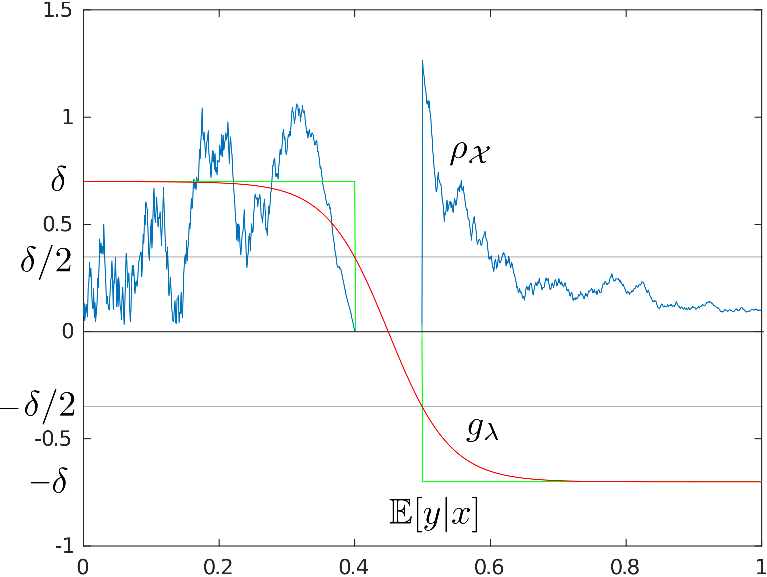
\includegraphics[width=0.5\textwidth]{figures/example.pdf}
  \caption{Pictorial representation of a model in $1$D satisfying Example~\ref{ex:independent-noise-on-labels}, ($p = 0.15$). Blue: $\rhox$, green: $\condexp{y}{x}$, red: $g_\la$.}
  \label{fig:example-A5}
  %
  %X = 0:0.001:1
  %y = rand(numel(X),1) - 0.5
  %cy = (4.*(1-25.0/4.0*X.^2).*(X <= 2/5.0) + exp(3-5*X).*(X >= 1/2));
  %plot(X, (abs(cumsum(y)) + 0.1).*cy'*1000/(3*a))
  %hold on
  %plot(X, 0.7*((X <=2/5) - (X >= 1/2)), 'g')
  %plot(X, 1.4./(1 + exp(-20.0*log(1/3.0).*(X-9/20.0))) - 0.7, 'r')
\end{figure}


\bpr{\bfseries of Proposition~\ref{prop:2g-makes-gstar}}
Since we are under \asm{asm:margin}, we can apply Prop.~\ref{prop:exists-gPN} that prove the existence two functions $q_{\mathcal{S}_+, \mathcal{S}_-}, q_{\mathcal{S}_-, \mathcal{S}_+} \in W^{s,2}$ with the property to be respectively equal to $1$ on $\mathcal{S}_+$, $0$ on $\mathcal{S}_-$, and $1$ on $\mathcal{S}_-$, $0$ on $\mathcal{S}_+$. 
Since $W^{s,2}$ is a Banach algebra \citep[see][]{adams2003sobolev}, then $g h \in W^{s,2}$ for any $g, h \in W^{s,2}$. So in particular 
$$g_\ast ~=~ g_+^*  q_{\mathcal{S}_+,\mathcal{S}_-} ~-~ g_-^*  q_{\mathcal{S}_-, \mathcal{S}_+},$$
belongs to $W^{s,2}$ (and so to $\hh$) and is equal to $\condexp{y}{x}$ a.e. on the support of $\rhox$ by definition. Finally, \asm{asm:flambda-correct-sign} is satisfied, by Prop.~\ref{prop:gstar-in-hh-gives-gla-good}.
\epr

\bpr{\bfseries of Example~\ref{ex:independent-noise-on-labels}}
By definition of $y$, we have that
$$\condexp{y}{x} = (1-2p)g(x), \quad g(x) = {\mathbf 1}_{\mathcal{S}_+} - {\mathbf 1}_{\mathcal{S}_-}.$$
In particular note that \asm{asm:separability} is satisfied with $\delta = 1-2p > 0$ since $p \in [0,1/2)$. Moreover note that  $\condexp{y}{x}$ is constant $\delta$ on $\mathcal{S}_+$ and $-\delta$ on $\mathcal{S}_-$. Note now that there exists two functions in $W^{s,2} \subseteq \hh$ (due to \asm{asm:kernel-rich}) that are, respectively $\delta$ on $\mathcal{S}_+$ and $-\delta$ on $\mathcal{S}_-$. They are exactly $g^*_+ := \delta q_{\mathcal{S}_+, \mathcal{S}_-}$ and $g^\ast_- = -\delta q_{\mathcal{S}_-, \mathcal{S}_+}$, from Prop.~\ref{prop:exists-gPN}. So we can apply Prop.~\ref{prop:2g-makes-gstar}, that given $g^\ast_+, g^*_-$ guarantees that \asm{asm:flambda-correct-sign} is satisfied. See an example in Figure \ref{fig:example-A5}.
\epr

\section{Preliminaries for Stochastic Gradient Descent}
\label{ap:SGDdevelopment}

In this section we show two preliminary results on stochastic gradient descent.

\subsection{Proof of the optimality condition on \texorpdfstring{$g_*$}{g*}}
\label{ap:optimality}

In this subsection we prove the optimality condition on $g_*$: $$\E \left[ \left(y_n - \Phg(x_n)\right)K_{x_n}\right] = 0.$$ Let us recall that as $\H$ is not necessarily dense in $L_2$, we have defined $\Phg$ as the orthonormal projector for the $L_2$ norm on $\H$ of $g_* = \E(y|x)$ which is the minimizer over all $g \in L_2$ of $\E (y - g(x) )^2$. Let $\F$ be the linear space $ \bar{\H}^{L_2}$ equipped with the $L_2$ norm, remark that $\Phg$ verifies $\Phg = \underset{g \in \F}{\text{argmin}} \| g-g_*  \|^2_{L_2}$ and that $g_* - \Phg = \mathcal{P}_{\H^\perp} (g_*) \in \F^\perp$.  

\begin{align*}
\E \left[ \left(y_n - \Phg(x_n)\right)K_{x_n}\right] &= \E \left[ \left(y_n - \E(y_n|x_n) + \E(y_n|x_n) - \Phg(x_n)\right)K_{x_n}\right] \\
&= \E \left[ \left(y_n - \E(y_n|x_n)\right)K_{x_n}\right] + \E \left[ \left(g_*(x_n) - \Phg(x_n)\right)K_{x_n}\right] \\
&= \E \left[\mathcal{P}_{\H^\perp} (g_*)(x_n)K_{x_n}\right] \\
&=0,
\end{align*}
%
where the last equality is true because we have $<\mathcal{P}_{\H^\perp} (g_*) , K(\cdot,z) >_{L_2} = 0$ and,
\begin{align*}
\|\E \left[\mathcal{P}_{\H^\perp} (g_*)(x_n)K_{x_n}\right]\|^2_\H &= \left\| \int_x \mathcal{P}_{\H^\perp} (g_*)(x)K_x d \rho(x) \right\|^2_\H  \\
&= \int_z \mathcal{P}_{\H^\perp} (g_*)(z) \left(\underbrace{\int_x \mathcal{P}_{\H^\perp} (g_*)(x)  K(x,z)  d \rho(x)}_{ = 0 }\right) d \rho(z) = 0.
\end{align*}

\subsection{Proof of Lemma~\ref{le:SGDrecursion}: reformulation of SGD as noisy recursion}
\label{ap:SGDreformulation}


Let $n \geqslant 1$ and $g_0 \in \H$, we start form the SGD recursion defined by \eqref{eq:firstSGD}:
\begin{align*}
{g}_n 
 & = {g}_{n-1} - \gamma_n  \big[ ( \langle K_{x_n} ,  {g}_{n-1}\rangle - y_n)K_{x_n}   + \lambda ({g}_{n-1} - g_0) \big] \\
 & = {g}_{n-1} - \gamma_n \big[ K_{x_n} \otimes K_{x_n} {g}_{n-1} - y_n K_{x_n}  + \lambda ({g}_{n-1} - g_0) \big] \\
 & = {g}_{n-1} - \gamma_n \big[ K_{x_n} \otimes K_{x_n} {g}_{n-1} - \Phg(x_n) K_{x_n} - \xi_n K_{x_n} + \lambda ({g}_{n-1} - g_0) \big] ,
 \end{align*}
 leading to (using the optimality conditions for $g_\lambda$ and $g_\ast$):
 \begin{align*}
{g}_n - g_\lambda 
  & =  {g}_{n-1} - g_\lambda - \gamma_n \big[ K_{x_n} \otimes K_{x_n} ( {g}_{n-1} - g_\lambda) + \lambda ({g}_{n-1} - g_0)  \\
   &   \hspace*{1.77cm} + (K_{x_n} \otimes K_{x_n}) g_\lambda - \Phg(x_n) K_{x_n} \big] + \gamma_n \xi_n K_{x_n} \\
 & = {g}_{n-1} - g_\lambda
 - \gamma_n \big[ K_{x_n} \otimes K_{x_n} ( {g}_{n-1} - g_\lambda)  + \lambda ({g}_{n-1} - g_0) \\
 &   \hspace*{1.77cm} 
 + (K_{x_n} \otimes K_{x_n} - \Sigma) g_\lambda + \Sigma g_\lambda  - \Phg(x_n) K_{x_n} \big] + \gamma_n \xi_n K_{x_n}\\
  & =  {g}_{n-1} - g_\lambda
 - \gamma_n \big[ K_{x_n} \otimes K_{x_n} ( {g}_{n-1} - g_\lambda)  + \lambda {g}_{n-1} 
 + (K_{x_n} \otimes K_{x_n} - \Sigma) g_\lambda \\
&   \hspace*{1.77cm} -\lambda g_\lambda + \E \left[ \Phg(x_n) K_{x_n} \right] - \Phg(x_n) K_{x_n} \big] + \gamma_n \xi_n K_{x_n}\\
 & =  {g}_{n-1} - g_\lambda
 - \gamma_n \big[ (  K_{x_n} \otimes K_{x_n} + \lambda I)( {g}_{n-1} - g_\lambda)   + (K_{x_n} \otimes K_{x_n} - \Sigma) g_\lambda \\
 &  \hspace*{1.77cm} +   \E \left[ \Phg(x_n) K_{x_n} \right] - \Phg(x_n) K_{x_n}   \big] + \gamma_n \xi_n K_{x_n}\\
& =  \big[
I - \gamma_n   (  K_{x_n} \otimes K_{x_n} + \lambda I ) \big]
  ( {g}_{n-1} - g_\lambda ) \\
&    \hspace*{1.77cm}   + \gamma_n \left[  \xi_n K_{x_n} +  ( \Sigma- K_{x_n} \otimes K_{x_n}) g_\lambda +   \Phg(x_n) K_{x_n} - \E \left[ \Phg(x_n) K_{x_n} \right] \right] \\ 
  & =  \big[
I - \gamma_n   (  K_{x_n} \otimes K_{x_n} + \lambda I ) \big]
  ( {g}_{n-1} - g_\lambda )\\
&    \hspace*{1.77cm}     + \gamma_n \left[  \xi_n K_{x_n}  - (K_{x_n} \otimes K_{x_n}) g_\lambda +   \Phg(x_n) K_{x_n} + \Sigma g_\lambda - \E \left[ \Phg(x_n) K_{x_n} \right] \right] \\ 
    & =  \big[
I - \gamma_n   (  K_{x_n} \otimes K_{x_n} + \lambda I ) \big]
  ( {g}_{n-1} - g_\lambda )  \\
&    \hspace*{1.77cm}   + \gamma_n \left[  \xi_n K_{x_n}   +   (\Phg(x_n)- g_\lambda(x_n)) K_{x_n} - \E \left[ (\Phg(x_n)- g_\lambda(x_n)) K_{x_n} \right] \right].
\end{align*}

\section{Proof of stochastic gradient descent results} \label{sec:AppSGD}

Let us recall for the Appendix the SGD recursion defined in Eq.~\eqref{eq:SGDabstract}: 
\begin{equation*}
   \eta_n = ( \idm - \gamma H_n) \eta_{n-1} + \gamma_n \varepsilon_n,
\end{equation*}
for which we assume \sgdasm{asm:init}, \sgdasm{asm:noise-iid}, \sgdasm{asm:noise-bound},\sgdasm{asm:weird-bound}, \sgdasm{asm:commute}.

\paragraph{Notations.}

We define the following notations, which will be useful during all the proofs of the section: 

\BIT
\item the following contractant operators:  for $i \geqslant k $, $$M(i,k) = (\idm - \gamma H_i ) \cdots ( \idm - \gamma H_k), \text{ and } M(i,i+1) = \idm, $$ 
\item the following sequences $Z_k = M(n,k+1) \varepsilon_k$ and $W_n = \sum_{k=1}^n \gamma_k  Z_k$. 
\EIT

then,
\begin{equation}
 \eta_n =
M(n,n) \eta_{n-1} + \gamma_n \varepsilon_n 
\end{equation}
\begin{equation}
\label{eq:decomposition}
 \eta_n = 
M(n,1)  \eta_0 + \sum_{k=1}^n \gamma_k M(n,k+1) \varepsilon_k,
\end{equation}

Note that in all this section, when there is no ambiguity, we will use $\|\cdot\|$ instead of $\|\cdot\|_\H$. 

\subsection{Non-averaged SGD - Proof of Theorem \ref{th:SGDalpha}}
\label{ap:SGDalpha}

In this section, we define the two following sequences: $\displaystyle \alpha_n = \prod_{i=1}^n ( 1-\gamma_i \lambda)$, \\ $\displaystyle \beta_n = \sum_{k=1}^n \gamma_k^2 \prod_{i=k+1}^n (1-\gamma_i \lambda)^2$ and $\zeta_n = \displaystyle \sup_{ k \leqslant n}\gamma_k \prod_{i=k+1}^n \left(1-\gamma_i\lambda\right)$.   

We can decompose $\eta_n$ in two terms: 
\begin{eqnarray}
 \eta_n = \underbrace{M(n,1) \eta_0}_{\textbf{Biais term}} + \underbrace{W_n}_{\textbf{Noise term}},
\end{eqnarray}
\BIT
\item The biais term represents the speed at which we forget initial conditions. It is the product of $n$ contracting operators $$\|  M(n,1)  \eta_0 \| \leqslant \prod_{i=1}^n ( 1-\gamma_i \lambda) \| \eta_0\| = \alpha_n \|\eta_0\|.$$
\item The noise term $W_n$ which is a martingale. We are going to show by using a concentration inequality that the probability of the event $\{ \| W_n \| \geq t\}$ goes to zero exponentially fast.
\EIT

\subsubsection{General result for all \texorpdfstring{$(\gamma_n)$}{gamma}}

As $W_n = \sum_{k=1}^n \gamma_k Z_k$, we want to apply Corollary \ref{Probabilisticcor} of section \ref{sec:proba} to $(\gamma_kZ_k)_{k \in \mathbb{N}}$ that is why we need the following lemma:

\begin{lemma}
\label{le:boundsalpha}
We have the following bounds: 
\begin{eqnarray}
\sup_{ k \leqslant n} \| \gamma_k Z_k \| &\leqslant& c^{1/2} \zeta_n, \ and \\
\sum_{k=1}^n \mathbb{E}\left[ \|\gamma_k Z_k\|^2 | \mathcal{F}_{k-1} \right] &\leqslant& \tr C \beta_n,
\end{eqnarray}
where $c$ and $C$ are defined by \sgdasm{asm:noise-bound}.
\end{lemma}

\begin{proof}
First, $ \|\gamma_k Z_k \| = \gamma_k \left\| M(n,k+1) \varepsilon_k \right\| \leq \gamma_k\left\| M(n,k+1) \right\|_{\text{op}} \left\| \varepsilon_k \right\| \leq \gamma_k\displaystyle \frac{\alpha_n}{\alpha_k} \left\| \varepsilon_k \right\| \leqslant \zeta_n c^{1/2} $. 

Second, 
\begin{eqnarray*}
\sum_{k=1}^n \mathbb{E}\left[ \|\gamma_k Z_k\|^2 | \mathcal{F}_{k-1} \right] 
&\leqslant& \sum_{k=1}^n \displaystyle \frac{\alpha_n^2}{\alpha_k^2}\ \gamma_k^2\  \E \left\| \varepsilon_k  \right\|^2 \\
&\leqslant& \sum_{k=1}^n \displaystyle \frac{\alpha_n^2}{\alpha_k^2}\ \gamma_k^2\  \tr C.
\end{eqnarray*}

Hence,
\begin{eqnarray*}
\sum_{k=1}^n \mathbb{E}\left[ \|\gamma_k Z_k\|^2 | \mathcal{F}_{k-1} \right]  &\leqslant& \sum_{k=1}^n \gamma_k^2 \prod_{i=k+1}^n (1-\gamma_i \lambda)^2 \tr C 
\\
&=&  \tr C \beta_n.      
\end{eqnarray*}
\end{proof}
\begin{proposition}
\label{prop:alphabetazeta}
We have the following inequality: for $t > 0, n \geqslant 1$,
\begin{eqnarray}
 \|\eta_n \| &\leqslant& \alpha_n \|\eta_0\| + V_n, \quad \text{with}\\
\P \left( V_n \geqslant t \right) &\leqslant& 2\exp \left( - \frac{t^2}{2(\tr C \beta_n + c^{1/2} \zeta_n t / 3)}  \right).
\end{eqnarray}
\end{proposition}
\begin{proof}
We just need to apply Lemma \ref{le:boundsalpha} and Corollary \ref{Probabilisticcor} to the martingale $W_n$ and $V_n = \|W_n\|$ for all $n$.
\end{proof}

\subsubsection{Result for \texorpdfstring{$\gamma_n = \gamma/n^\alpha$}{gamma} }

We now derive estimates of $\alpha_n, \beta_n$ and $\zeta_n$ to have explicit bound for the previous result in the case where $\gamma_n = \displaystyle \frac{\gamma}{n^\alpha}$ for $\alpha \in [0,1]$. Some of the estimations are taken from \citet{gradsto}.

\begin{lemma}
\label{le:nalpha}
In the interesting particular case where $\gamma_n = \displaystyle \frac{\gamma}{n^\alpha}$ for $\alpha \in [0,1]$:
\BIT
\item for $\alpha = 1,\ i.e \ \gamma_n=\displaystyle \frac{\gamma}{n}$, then $\zeta_n = \displaystyle \frac{\gamma}{1-\gamma\lambda}\alpha_n$, and we have the following estimations for $\gamma\lambda < 1/2$: \\(i)\ ~$\alpha_n \leqslant \displaystyle \frac{1}{n^{\gamma\lambda}}$, (ii)\ ~$\beta_n \leqslant \displaystyle \frac{2(1-\gamma\lambda)}{1-2\gamma\lambda} \frac{4^{\gamma\lambda}\gamma^2}{n^{2\gamma\lambda}}$, (iii)\ ~$ \zeta_n \leqslant \displaystyle \frac{\gamma}{(1-\lambda\gamma)n^{\gamma\lambda}}$.
\item for $\alpha = 0,\ i.e \ \gamma_n=\displaystyle \gamma$, then $\zeta_n = \gamma$, and we have the following: \\(i)\ ~$\alpha_n = (1-\gamma\lambda)^n$, (ii)\ ~$\beta_n \leqslant \displaystyle \frac{\gamma}{\lambda}$, (iii)\ ~$ \zeta_n = \gamma$.
\item for $\alpha \in \left]0,1\right[,\ \zeta_n=\max\left\{ \gamma_n, \displaystyle \frac{\gamma}{1-\gamma\lambda}\alpha_n \right\}$, and we have the following estimations: 

(i)\ ~$\alpha_n \leqslant \displaystyle \exp\left(  -\frac{\gamma\lambda}{1-\alpha}\left( (n+1)^{1-\alpha} -1  \right)   \right)$, 

(ii) Denoting $ L_\alpha = \frac{2\lambda\gamma}{1-\alpha} 2^{1-\alpha}\left( 1-\left(\frac{3}{4}\right)^{1-\alpha} \right)$, we distinguish three cases:  
\BIT
\item $\alpha >1/2$, \ ~$\beta_n \leqslant \gamma^2\frac{2\alpha}{2\alpha-1} \exp\left( -L_\alpha n^{1-\alpha}\right) +  \frac{2^\alpha\gamma}{\lambda n^\alpha}$,
\item $\alpha = 1/2$, \ ~$\beta_n \leqslant \gamma^2\ln (3n) \exp\left( -L_\alpha n^{1-\alpha}\right) +  \frac{2^\alpha\gamma}{\lambda n^\alpha}$,
\item $\alpha  < 1/2$, \ ~$\beta_n \leqslant \gamma^2\frac{n^{1-2\alpha}}{1- 2\alpha} \exp\left( -L_\alpha n^{1-\alpha}\right) +  \frac{2^\alpha\gamma}{\lambda n^\alpha}$.
\EIT
(iii)\ ~$ \zeta_n \leqslant \max \left\{\frac{\gamma}{1-\gamma\lambda}\exp\left(  -\frac{\gamma\lambda}{1-\alpha}\left( (n+1)^{1-\alpha} -1  \right)   \right), \frac{\gamma}{n^\alpha} \right\}.$
\EIT

Note that in this case for $n$ large enough we have the following estimations: 

(i)\ ~$\alpha_n \leqslant \displaystyle \exp\left(  -\frac{\gamma\lambda}{2^{1-\alpha}(1-\alpha)}n^{1-\alpha}    \right)$, (ii)\ ~$\beta_n \leqslant \displaystyle \frac{2^{\alpha+1}\gamma}{\lambda n^\alpha}$, (iii)\ ~$ \zeta_n \leqslant \displaystyle \frac{\gamma}{n^{\alpha}}$.
\end{lemma}

\begin{proof}
First we show for $\alpha \in [0,1]$ the equality for $\zeta_n$.
Denote $a_k = \gamma_k \prod_{i=k+1}^n (1-\gamma_i\lambda)$, we want to find $\zeta_n = \sup_{k \leqslant n} a_k$. We show for $\gamma_n = \displaystyle \frac{\gamma}{n^\alpha}$ that $(a_k)_{k\geqslant 1 }$ decreases then increases so that $\zeta_n = \max\{ a_1 , a_n \}$.
Let $k \leqslant n-1$, 
\begin{eqnarray*}
\frac{a_{k+1}}{a_k}&=&\frac{\gamma_{k+1}}{\gamma_k}\frac{1}{(1-\gamma_{k+1}\lambda)}\\
&=&\frac{1}{\frac{\gamma_{k}}{\gamma_{k+1}}-\gamma_{k}\lambda}\\
\end{eqnarray*}
Hence, $\displaystyle \frac{a_{k}}{a_{k+1}} - 1 = \frac{\gamma_{k}}{\gamma_{k+1}}-\gamma_{k}\lambda-1$. Take $\alpha \in \left]0,1\right[$, in this case where $\gamma_n = \displaystyle \frac{\gamma}{n^\alpha}$, 

$$ \frac{a_{k}}{a_{k+1}} - 1 = \left(1+\frac{1}{k}\right)^\alpha - \frac{\gamma\lambda}{k^\alpha}-1 .$$

A rapid study of the function $\displaystyle f_\alpha(x) = \left(1+\frac{1}{x}\right)^\alpha - \frac{\gamma\lambda}{x^\alpha}-1$ in $\mathbb{R}_+^\star$ shows that it decreases until $x_\star = \left( \gamma \lambda\right)^{\frac{1}{(\alpha-1)}}-1$ then increases. This concludes the proof for $\alpha \in \left]0,1\right[$. By a direct calculation for $\alpha = 1$, $\displaystyle \frac{a_{k}}{a_{k+1}} - 1 = \frac{1-\gamma\lambda}{k} \geqslant 0$ thus $a_k$ is non increasing and $\zeta_n =a_1 = \displaystyle \frac{\gamma}{1-\gamma\lambda}\alpha_n$. Similarly, for $\alpha=0$, $\displaystyle \frac{a_{k}}{a_{k+1}} - 1 = \gamma\lambda < 0$ thus $a_k$ is increasing and $\zeta_n =a_n = \gamma_n$.

We show now the different estimations we have for $\alpha_n$, $\beta_n$ and $\zeta_n$ for the three cases above.
\BIT
\item for $\alpha = 1$, 
\begin{eqnarray*}
\ln \alpha_n &=& \sum_{i=1}^n \ln \left( 1 - \frac{\gamma \lambda}{i}\right) \leqslant -\gamma \lambda \sum_{i=1}^n \frac{1}{i} \leqslant -\gamma\lambda \ln n \\
\alpha_n &\leqslant& \frac{1}{n^{\gamma \lambda}}.
\end{eqnarray*}
Then, 
\begin{eqnarray*}
\beta_n &=& \gamma^2 \sum_{k=1}^n \frac{1}{k^2}\prod_{i=k+1}^n \left( 1-\frac{\gamma\lambda}{i} \right)^2 \\
\beta_n &\leqslant& \gamma^2 \sum_{k=1}^n \frac{1}{k^2}\exp\left( -2 \gamma\lambda \sum_{i=k+1}^n \frac{1}{i}  \right) \\
&\leqslant& \gamma^2 \sum_{k=1}^n \frac{1}{k^2}\exp\left( -2 \gamma\lambda \ln\left( \frac{n+1}{k+1} \right)  \right) \\
&\leqslant& \gamma^2 \sum_{k=1}^n \frac{1}{k^2}\left( \frac{k+1}{n+1} \right)^{2\gamma\lambda}  \\
&\leqslant& 4^{\gamma\lambda}\gamma^2 \sum_{k=1}^n \frac{1}{k^2}\left( \frac{k}{n} \right)^{2\gamma\lambda}  \\
&\leqslant& \frac{4^{\gamma\lambda}\gamma^2}{n^{2\gamma\lambda}} \sum_{k=1}^n k^{2\gamma\lambda-2},
\end{eqnarray*}
Moreover for $\displaystyle \gamma\lambda < \frac{1}{2},\  \sum_{k=1}^n k^{2\gamma\lambda-2} \leqslant 1 - \frac{1}{2\gamma\lambda-1} = \frac{2(1-\gamma\lambda)}{1-2\gamma\lambda}$, hence,

\begin{eqnarray*}
\beta_n &\leqslant&  \frac{2(1-\gamma\lambda)}{1-2\gamma\lambda} \frac{4^{\gamma\lambda}\gamma^2}{n^{2\gamma\lambda}}
\end{eqnarray*}

Finally,
\begin{eqnarray*}
\zeta_n = \frac{\gamma}{1-\gamma\lambda} \alpha_n \leqslant \frac{\gamma}{1-\gamma\lambda} \frac{1}{n^{\gamma\lambda}}.
\end{eqnarray*}

\item for $\alpha = 0$, 
\begin{eqnarray*}
\alpha_n = \prod_{i=1}^n \left( 1 - \gamma \lambda\right) = (1-\gamma\lambda)^n.
\end{eqnarray*}
Then, 
\begin{eqnarray*}
\beta_n = \gamma^2 \sum_{k=1}^n \prod_{i=k+1}^n \left( 1-\gamma\lambda \right)^2 = \gamma^2 \sum_{k=1}^n \left( 1- \gamma\lambda \right)^{2(n-k)} \leqslant \frac{1}{1-(1-\lambda\gamma)^2} \leqslant \frac{\gamma}{\lambda}.
\end{eqnarray*}
Finally,
\begin{eqnarray*}
\zeta_n = \gamma_n = \gamma.
\end{eqnarray*}

\item for $\alpha \in ]0,1[$, 
\begin{eqnarray*}
\ln \alpha_n &=& \sum_{i=1}^n \ln \left( 1 - \frac{\gamma \lambda}{i^\alpha}\right) \leqslant -\gamma \lambda \sum_{i=1}^n \frac{1}{i^\alpha} \leqslant -\gamma\lambda \frac{(n+1)^{1-\alpha}-1}{1-\alpha} \\
\alpha_n &\leqslant& \exp\left( -\frac{\gamma\lambda}{1-\alpha} \left((n+1)^{1-\alpha}-1\right) \right).
\end{eqnarray*}
To have an estimation on $\beta_n$, we are going to split it into two sums. Let $m \in \llbracket 1,n \rrbracket$,
\begin{align*}
\beta_n &= \sum_{k=1}^n \gamma_k^2\prod_{i=k+1}^n \left( 1-\gamma_i\lambda \right)^2 = \sum_{k=1}^{m} \gamma_k^2\prod_{i=k+1}^n \left( 1-\gamma_i\lambda \right)^2 +  \sum_{k=m+1}^n \gamma_k^2\prod_{i=k+1}^n \left( 1-\gamma_i\lambda \right)^2\\
\beta_n &\leqslant \sum_{k=1}^m  \gamma_k^2 \exp\left( -2 \lambda \sum_{i=m+1}^n \gamma_i  \right) +  \frac{\gamma_m}{\lambda}\sum_{k=m+1}^n \prod_{i=k+1}^n \left( 1-\gamma_i\lambda \right)^2 \lambda\gamma_k\\
 &\leqslant \sum_{k=1}^n  \gamma_k^2 \exp\left( -2 \lambda \sum_{i=m+1}^n \gamma_i  \right) \\
 & \hspace{2.98cm}+  \frac{\gamma_m}{\lambda}\sum_{k=m+1}^n \left[ \prod_{i=k+1}^n \left( 1-\gamma_i\lambda \right)^2 - \prod_{i=k+1}^n \left( 1-\gamma_i\lambda \right)^2 (1-\gamma_k\lambda)  \right]\\
 &\leqslant \sum_{k=1}^n  \gamma_k^2 \exp\left( -2 \lambda \sum_{i=m+1}^n \gamma_i  \right) +  \frac{\gamma_m}{\lambda}\sum_{k=m+1}^n \left[ \prod_{i=k+1}^n \left( 1-\gamma_i\lambda \right)^2 - \prod_{i=k}^n \left( 1-\gamma_i\lambda \right)^2 \right]\\
 &\leqslant \sum_{k=1}^n  \gamma_k^2 \exp\left( -2 \lambda \sum_{i=m+1}^n \gamma_i  \right) +  \frac{\gamma_m}{\lambda} \left(1- \prod_{i=m+1}^n \left( 1-\gamma_i\lambda \right)^2\right) \\
 &\leqslant \sum_{k=1}^n  \gamma_k^2 \exp\left( -2 \lambda \sum_{i=m+1}^n \gamma_i  \right) +  \frac{\gamma_m}{\lambda}.
\end{align*}
By taking $\gamma_n = \displaystyle \frac{\gamma}{n^\alpha}$ and $ m = \displaystyle \lfloor\frac{n}{2}\rfloor $, we get: 
\begin{eqnarray*}
\beta_n &\leqslant& \gamma^2\sum_{k=1}^n  \frac{1}{k^{2\alpha}} \exp\left( -2 \lambda\gamma \sum_{i=\lfloor\frac{n}{2}\rfloor+1}^n \frac{1}{i^{\alpha}}  \right) +  \frac{2^\alpha\gamma}{\lambda n^\alpha} \\
 &\leqslant& \gamma^2\sum_{k=1}^n  \frac{1}{k^{2\alpha}} \exp\left( -\frac{2 \lambda\gamma}{1-\alpha} \left( \left(n+1\right)^{1-\alpha}-\left(\frac{n}{2}+1\right)^{1-\alpha} \right) \right) +  \frac{2^\alpha\gamma}{\lambda n^\alpha} \\
  &\leqslant& \gamma^2\sum_{k=1}^n  \frac{1}{k^{2\alpha}} \exp\left( -\frac{2 \lambda\gamma}{1-\alpha} n^{1-\alpha} \left( \left(1+\frac{1}{n}\right)^{1-\alpha}-\left(\frac{1}{2}+\frac{1}{n}\right)^{1-\alpha} \right) \right) +  \frac{2^\alpha\gamma}{\lambda n^\alpha} \\
  &\leqslant& \gamma^2\sum_{k=1}^n  \frac{1}{k^{2\alpha}} \exp\left( -\frac{2 \lambda\gamma}{1-\alpha} n^{1-\alpha} 2^{1-\alpha}\left( 1-\left(\frac{3}{4}\right)^{1-\alpha} \right)\right) +  \frac{2^\alpha\gamma}{\lambda n^\alpha} .
\end{eqnarray*}
Calling $S_n^\alpha = \sum_{k=1}^n \frac{1}{k^{2\alpha}}$ and noting that: for $\alpha > 1/2,\ S_n^\alpha \leqslant \frac{2\alpha}{2\alpha - 1}$, $\alpha = 1/2,\ S_n^\alpha \leqslant \ln(3n)$ and $\alpha < 1/2,\ S_n^\alpha \leqslant \frac{n^{1-2\alpha}}{1 - 2\alpha }$ we have the expected result.

Finally,
\begin{eqnarray*}
\zeta_n \leqslant \max \left\{\frac{\gamma}{1-\gamma\lambda}\exp\left(  -\frac{\gamma\lambda}{1-\alpha}\left( (n+1)^{1-\alpha} -1  \right)   \right), \frac{\gamma}{n^\alpha} \right\}.
\end{eqnarray*}
\EIT

\end{proof}

With this estimations we can easily show the Theorem \ref{th:SGDalpha}. In the following we recall the main result of this Theorem and give an extension for $\alpha = 0$ and $\alpha = 1$ that cannot be found in the main text.

\begin{proposition}[SGD, decreasing step size: $\gamma_n = \gamma/n^\alpha$]
\label{prop:fullalpha}
Assume \sgdasm{asm:init}, \sgdasm{asm:noise-iid}, \sgdasm{asm:noise-bound}, $\gamma_n = \gamma/n^\alpha$, $\gamma\lambda < 1$ and denote by $\eta_n \in \H$ the n-th iterate of the recursion in Eq. \eqref{eq:SGDabstract}. We have for $t > 0, n \geqslant 1$,
\BIT
\item for $\alpha = 1$ and $\gamma\lambda < 1/2$, $\displaystyle \ \|g_n - g_\lambda\|_\H \leqslant \frac{\|g_0 - g_\lambda\|_\H}{n^{\gamma\lambda}}  +V_n,$ almost surely, with
 \begin{align*}
\P \left(V_n  \geqslant t\right) \leqslant 2\exp\left(-\frac{t^2}{4^{3/2}(\tr C) \gamma^2/((1-2\gamma\lambda) n ^{\gamma\lambda}) +4tc^{1/2}\gamma/3  }\cdot n^{\gamma\lambda}\right);
\end{align*}
\item for $\alpha = 0$, $\displaystyle \ \|g_n - g_\lambda\|_\H \leqslant (1-\gamma\lambda)^n \|g_0 - g_\lambda\|_\H + V_n$, almost surely, with
$$\P \left( V_n \geqslant t \right) \leqslant 
2\exp\left( -\frac{t^2}{2\gamma(\tr C  / \lambda + t c^{1/2} / 3 )}\right);$$

\item for $\alpha \in (0,1)$, $\|g_n - g_\lambda\|_\H \leqslant \exp\left(  -\frac{\gamma\lambda}{1-\alpha}\left( (n+1)^{1-\alpha} -1  \right)   \right) \|g_0 - g_\lambda\|_\H + V_n$, almost surely for $n$ large enough \footnote {See Appendix Section \ref{sec:AppSGD} Lemma \ref{le:nalpha} for more details.}, with
$$\P \left( V_n \geqslant t \right) \leqslant 2\exp\left( -\frac{ t^2 }{ \gamma (2 ^{\alpha + 2} \tr C/\lambda  + 2 c^{1/2}t  / 3)}\cdot n^{\alpha}\right).$$
\EIT
\end{proposition}

\begin{proof}[Proof of Theorem~\ref{th:SGDalpha}]
We apply Proposition \ref{prop:alphabetazeta}, and the bound found on $\alpha_n$, $\beta_n$ and $\zeta_n$ in Lemma \ref{le:nalpha} to get the results.
\end{proof}



\subsection{Averaged SGD for the variance term \texorpdfstring{($\eta_0 = 0$)}{} - Proof of Theorem \ref{th:SGDaveraged}}
\label{ap:SGDaverage}

We consider the same recursion but with $\gamma_n = \gamma$:
$$
\eta_n = ( \idm - \gamma H_n) \eta_{n-1} + \gamma \varepsilon_n,
$$
started at  $\eta_0=0$ and with assumptions \sgdasm{asm:init}, \sgdasm{asm:noise-iid}, \sgdasm{asm:noise-bound},\sgdasm{asm:weird-bound}, \sgdasm{asm:commute}.

However, in this section, we consider the averaged: 
$$
\bar{\eta}_n = \frac{1}{n+1} \sum_{i=0}^n \eta_i.
$$

Thus, we get
$$
\bar{\eta}_n = \frac{1}{n+1} \sum_{i=0}^n \gamma \sum_{k=1}^i M(i,k+1) \varepsilon_k
= \frac{\gamma}{n+1} 
 \sum_{k=1}^n \Big( \sum_{i=k}^n M(i,k+1) \Big) \varepsilon_k
 = \frac{\gamma}{n+1}  \sum_{k=1}^n \bar{Z}_k.
 $$

Our the goal is to bound $\displaystyle\P \left( \left\| \bar{\eta}_n  \right\| \geqslant t \right) $ using Propostion \ref{Probabilisticprop} that is going to lead us to some Bernstein concentration inquality. Calling, as above, $\displaystyle \bar{Z}_k =  \sum_{i=k}^n M(i,k+1) \varepsilon_k$, and as $\E \left[ \bar{Z}_k | \mathcal{F}_{k-1} \right] = 0$ we just need to bound, $\sup_{k \leqslant n} \| \bar{Z}_k \|$ and $\sum_{k = 1}^n \E \left[ \|\bar{Z}_k\|^2 | \mathcal{F}_{k-1} \right] $. For a more general result, we consider in the following lemma $\displaystyle (A^{1/2}\bar{Z}_k)_k$.

\begin{lemma}
\label{le:averagebounds}
Assuming \sgdasm{asm:init}, \sgdasm{asm:noise-iid}, \sgdasm{asm:noise-bound},\sgdasm{asm:weird-bound}, \sgdasm{asm:commute}, we have the following bounds for $\displaystyle \bar{Z}_k =  \sum_{i=k}^n M(i,k+1) \varepsilon_k$: 
\begin{align}
\sup_{k \leqslant n} \| A^{1/2} \bar{Z}_k \| &\leqslant \frac{c^{1/2} \|A\|_{op}^{1/2} }{\gamma \lambda} \\
\sum_{k = 1}^n \E \left[ \|A^{1/2} \bar{Z}_k\|^2 | \mathcal{F}_{k-1} \right] &\leqslant n \frac{1}{\gamma^2}\frac{1}{1-\gamma/2\gamma_0} \tr \left(A H^{-2}\cdot C \right).
\end{align}

\end{lemma}

\begin{proof}
First $\| A^{1/2} \bar{Z}_k \| \leqslant \|A\|_{op}^{1/2} \| \bar{Z}_k \|$ and we have, almost surely, $\| \varepsilon_k  \| \leqslant c^{1/2} $ and $ H_n \succcurlyeq \lambda \idm $, thus for all $k$, as $\gamma\lambda \leqslant 1$, $\idm - \gamma H_k \preccurlyeq (1-\gamma\lambda) \idm$. Hence,  $\| M(i,k+1) \|_{\textrm {op}} \leqslant ( 1- \gamma \lambda)^{i-k}$ and,
$$ \| \bar{Z}_k \| \leqslant \|\varepsilon_k\| \sum_{i=k}^n \| M(i,k+1) \|_{\textrm {op}}
 \leqslant
c^{1/2} \sum_{i=k}^n ( 1- \gamma \lambda)^{i-k} 
 \leqslant
\frac{c^{1/2} }{\gamma \lambda}
 $$
Second, we need an upper bound on $\displaystyle \E \left[ \|A^{1/2}\bar{Z}_k\|^2 | \mathcal{F}_{k-1} \right]$, we are going to find it in two steps: 
\BIT
\item \textbf{Step 1:} we first show that the upper bound depends of the trace of some operator involving~$H^{-1}$. \begin{eqnarray*}
\E \left[ \|A^{1/2} \bar{Z}_k\|^2 | \mathcal{F}_{k-1} \right]
& \leqslant & 2 \sum_{i=k}^n \tr\left( A \left(\gamma H\right)^{-1}\E \left[    M(i,k+1) C {M(i,k+1)}^*\right] \right),
\end{eqnarray*} 
\item \textbf{Step 2:} we then upperbound this sum to a telescopic one involving $H^{-2}$ to finally show: \begin{eqnarray*}
\E \left[ \|A^{1/2} \bar{Z}_k\|^2 | \mathcal{F}_{k-1} \right]
& \leqslant & \frac{1}{\gamma^2}\frac{1}{1-\gamma/2\gamma_0} \tr \left(AH^{-2} C \right).
\end{eqnarray*} 
\EIT

\paragraph{Step 1:} We write,

\begin{eqnarray*}
\E \left[ \|A^{1/2} \bar{Z}_k\|^2 | \mathcal{F}_{k-1} \right] & =& \E \left[ \sum_{k\leqslant i, j \leqslant n} \left\langle A^{1/2} M(i,k+1)\varepsilon_k, A^{1/2} M(j,k+1)\varepsilon_k\right\rangle | \mathcal{F}_{k-1} \right] \\
& =& \E \left[ \sum_{k\leqslant i, j \leqslant n} \left\langle M(i,k+1)\varepsilon_k, A M(j,k+1)\varepsilon_k\right\rangle | \mathcal{F}_{k-1} \right] \\
& =& \sum_{k\leqslant i, j \leqslant n} \E \left[ \tr \left( M(i,k+1)^* A M(j,k+1) \cdot \varepsilon_k\otimes \varepsilon_k\right) \right] \\
& =& \sum_{k\leqslant i, j \leqslant n} \tr\left( \E \left[  M(i,k+1)^* A M(j,k+1)\right] \cdot \E \left[ \varepsilon_k\otimes \varepsilon_k \right]\right).
\end{eqnarray*}
We have $\E \left[ \varepsilon_k\otimes \varepsilon_k \right] \preccurlyeq C $ so that as every operators are positive semi-definite, 
\begin{eqnarray*}
\E \left[ \|A^{1/2} \bar{Z}_k\|^2 | \mathcal{F}_{k-1} \right] & \leqslant & \sum_{k\leqslant i, j \leqslant n} \tr\left( \E \left[  M(i,k+1)^* A M(j,k+1)\right] \cdot C\right).
\end{eqnarray*}
We now bound the last expression by dividing it into two terms, noting $M(i,k) = M^i_k$ for more compact notations (only until the end of the proof),
\begin{align*}
\sum_{k\leqslant i, j \leqslant n} \tr\left( \E \left[  {M^i_{k+1}}^* A M^j_{k+1}\right] \cdot C\right) & = \sum_{i=k}^n \tr\left( \E \left[  {M^i_{k+1}}^* A M^i_{k+1}\right] \cdot C\right) \\
& \hspace{2cm}+ 2 \sum_{k\leqslant i < j \leqslant n} \tr\left( \E \left[  {M^i_{k+1}}^* A M^j_{k+1}\right] \cdot C\right).
\end{align*}
Moreover, 
\begin{eqnarray*}
 & &  \sum_{k\leqslant i < j \leqslant n} \tr\left( \E \left[  {M^i_{k+1}}^* A M^j_{k+1}\right] \cdot C\right) 
 \\ & = &  \sum_{k\leqslant i < j \leqslant n} \tr\left( \E \left[  {M^i_{k+1}}^* A \left( \idm - \gamma H \right)^{j-i} M^i_{k+1}\right] \cdot C\right) \\
& = &  \sum_{i=k}^n \tr\left( \E \left[  {M^i_{k+1}}^* A \sum_{j=i+1}^n \left( \idm - \gamma H \right)^{j-i} M^i_{k+1}\right] \cdot C\right) \\
& = &  \sum_{i=k}^n \tr\left( \E \left[  {M^i_{k+1}}^* A \left[ \left( \idm - \gamma H \right) \left( \idm - \left( \idm - \gamma H \right)^{n-i} \right) \left(\gamma H \right)^{-1} \right] M^i_{k+1}\right] \cdot C \right) \\
& \leqslant  &  \sum_{i=k}^n \tr\left( \E \left[  {M^i_{k+1}}^* A \left[ \left(\gamma H\right)^{-1} - \idm \right] M^i_{k+1}\right] \cdot C \right)\\
& \leqslant  &  \sum_{i=k}^n \tr\left( \E \left[  {M^i_{k+1}}^* A \left(\gamma H\right)^{-1} M^i_{k+1}\right] \cdot C \right)-\sum_{i=k}^n \tr\left( \E \left[  {M^i_{k+1}}^* A M^i_{k+1}\right] \cdot C \right).
\end{eqnarray*}
Hence, 

\eqals{
\sum_{k\leqslant i, j \leqslant n} \tr & \left( \E \left[  {M^i_{k+1}}^* A M^j_{k+1}\right] \cdot C\right)  \\
& = \sum_{i=k}^n \tr\left( \E \left[  {M^i_{k+1}}^* A M^i_{k+1}\right] \cdot C\right)
+ 2 \sum_{k\leqslant i < j \leqslant n} \tr\left( \E \left[  {M^i_{k+1}}^* A M^j_{k+1}\right] \cdot C\right) \\
& \leqslant  2 \sum_{i=k}^n \tr\left( \E \left[  {M^i_{k+1}}^* A \left(\gamma H\right)^{-1} M^i_{k+1}\right] \cdot C \right)- \sum_{i=k}^n \tr\left( \E \left[  {M^i_{k+1}}^* A M^i_{k+1}\right] \cdot C \right) \\
& \leqslant 2 \sum_{i=k}^n \tr\left( \E \left[  {M^i_{k+1}}^* A \left(\gamma H\right)^{-1} M^i_{k+1}\right] \cdot C \right)\\
& \leqslant 2 \sum_{i=k}^n \tr\left(A\left(\gamma H\right)^{-1}  \E \left[   M^i_{k+1} C {M^i_{k+1}}^*  \right] \right)
}

This concludes step 1.

\paragraph{Step 2: } Let us now try to bound $\displaystyle \sum_{i=k}^n \tr\left( A \left(\gamma H\right)^{-1}\E \left[    M^i_{k+1} C {M^i_{k+1}}^*\right] \right)$. We will do so by bounding it by a telescopic sum. Indeed,
\eqals{
&\E \left[  {M^{i+1}_{k+1}}C\left(\gamma H\right)^{-1}{M^{i+1}_{k+1}}^*\right]  = \E \left[  {M^{i}_{k+1}}\left(\idm - \gamma H_{i+1}\right)C\left(\gamma H\right)^{-1}\left(\idm - \gamma H_{i+1}\right){M^{i}_{k+1}}^*\right] \\
& = \E \left[  {M^{i}_{k+1}}\E \left[ C\left(\gamma H\right)^{-1} - C H^{-1} H_{i+1}- H_{i+1} C H^{-1} + \gamma H_{i+1}C H^{-1}H_{i+1} \right]{M^{i}_{k+1}}^*\right] \\
& = \E \left[  {M^{i}_{k+1}}C\left(\gamma H\right)^{-1}{M^{i}_{k+1}}^*\right]-2\E \left[  {M^{i}_{k+1}}C{M^{i}_{k+1}}^*\right]  + \gamma\E \left[  {M^{i}_{k+1}}\E \left[ H_{i+1}CH^{-1}H_{i+1} \right]{M^{i}_{k+1}}^*\right],
}
such that, by multiplying the previous equality by $A \left(\gamma H\right)^{-1}$ and taking the trace we have, 
\begin{align*}
\tr\left( A \left(\gamma H\right)^{-1}\E \left[  {M^{i+1}_{k+1}}C\left(\gamma H\right)^{-1}{M^{i+1}_{k+1}}^*\right]\right) &=  \tr\left(A \left(\gamma H\right)^{-1}\E \left[  {M^{i}_{k+1}}C\left(\gamma H\right)^{-1}{M^{i}_{k+1}}^*\right]\right)\\
 &-2\tr\left(A \left(\gamma H\right)^{-1}\E \left[  {M^{i}_{k+1}}C{M^{i}_{k+1}}^*\right]\right) \\
&+ \gamma \tr\left(A \left(\gamma H\right)^{-1}\E \left[  {M^{i}_{k+1}}\E \left[ H_{i+1}CH^{-1}H_{i+1} \right]{M^{i}_{k+1}}^*\right]\right),
\end{align*}
And as $\E \Big[  H_k C H^{-1} H_k \Big] \preccurlyeq \gamma_0^{-1} C$ we have, 
$$\gamma\tr\left(A \left(\gamma H\right)^{-1} \E \left[  {M^{i}_{k+1}}\E \left[ H_{i+1}CH^{-1}H_{i+1} \right]{M^{i}_{k+1}}^*\right]\right) \leqslant \gamma / \gamma_0 \tr\left(A \left(\gamma H\right)^{-1} \E \left[  {M^{i}_{k+1}}C{M^{i}_{k+1}}^*\right]\right), $$
thus,
\begin{eqnarray*}
\tr\left(A \left(\gamma H\right)^{-1} \E \left[ {M^{i+1}_{k+1}}C\left(\gamma H\right)^{-1}{M^{i+1}_{k+1}}^*\right]\right) &\leqslant&  \tr\left(A \left(\gamma H\right)^{-1}\E \left[  {M^{i}_{k+1}}C\left(\gamma H\right)^{-1}{M^{i}_{k+1}}^*\right]\right) \\
&-&2\tr\left(A \left(\gamma H\right)^{-1}\E \left[  {M^{i}_{k+1}}C{M^{i}_{k+1}}^*\right]\right) \\
& + & \gamma / \gamma_0 \tr\left(A \left(\gamma H\right)^{-1} \E \left[  {M^{i}_{k+1}}C{M^{i}_{k+1}}^*\right]\right)
\end{eqnarray*}
\begin{align*}
&\tr\left(A \left(\gamma H\right)^{-1} \E \left[  {M^{i}_{k+1}}C{M^{i}_{k+1}}^*\right]\right)\\ 
 &\leqslant \frac{1}{2-\frac{\gamma}{\gamma_0}} \left(\tr\left(A \left(\gamma H\right)^{-1}\E \left[  {M^{i}_{k+1}}C\left(\gamma H\right)^{-1}{M^{i}_{k+1}}^*\right]\right) - \tr\left(A \left(\gamma H\right)^{-1} \E \left[ {M^{i+1}_{k+1}}C\left(\gamma H\right)^{-1}{M^{i+1}_{k+1}}^*\right]\right)\right).
\end{align*}
If we take all the calculations from the beginning,
\begin{eqnarray*}
\E \left[ \|A^{1/2} \bar{Z}_k\|^2 | \mathcal{F}_{k-1} \right] & \leqslant & \sum_{k\leqslant i, j \leqslant n} \tr\left( \E \left[  {M^i_{k+1}}^* A M^j_{k+1}\right] \cdot C\right) \\
& \leqslant & 2 \sum_{i=k}^n \tr\left(A \left(\gamma H\right)^{-1} \E \left[  {M^{i}_{k+1}}C{M^{i}_{k+1}}^*\right]\right)\\
& \leqslant & \frac{2}{2-\gamma/\gamma_0} \sum_{i=k}^n \tr\left(A \left(\gamma H\right)^{-1}\E \left[  {M^{i}_{k+1}}C\left(\gamma H\right)^{-1}{M^{i}_{k+1}}^*\right]\right) \\
& &   \hspace*{1.77cm} -\tr\left(A \left(\gamma H\right)^{-1} \E \left[ {M^{i+1}_{k+1}}C\left(\gamma H\right)^{-1}{M^{i+1}_{k+1}}^*\right]\right)\\
& \leqslant & \frac{2}{2-\gamma/\gamma_0} \tr\left(A \left(\gamma H\right)^{-1}\E \left[  {M^{k}_{k+1}}C\left(\gamma H\right)^{-1}{M^{k}_{k+1}}^*\right]\right)\\
& \leqslant & \frac{1}{\gamma^2}\frac{1}{1-\gamma/2\gamma_0} \tr \left(A H^{-2}\cdot C \right),
\end{eqnarray*}
which concludes the proof if we sum this inequality from $1$ to $n$.

\end{proof}

We can now prove Theorem~\ref{th:SGDaveraged}:

\begin{proof}[Proof of Theorem~\ref{th:SGDaveraged}]
We apply Corollary \ref{Probabilisticcor} to the sequence $\left(\displaystyle\frac{\gamma}{n+1} A^{1/2}Z_k\right)_{k \leqslant n}$ thanks to Lemma \ref{le:averagebounds}. We have:
\begin{eqnarray*}
\sup_{k \leqslant n} \| \frac{\gamma}{n+1} A^{1/2}Z_k \| &\leqslant& \frac{c^{1/2} \|A^{1/2}\| }{(n+1) \lambda} \\
\sum_{k = 1}^n \E \left[ \|\frac{\gamma}{n+1} A^{1/2} Z_k\|^2 | \mathcal{F}_{k-1} \right] &\leqslant& \frac{1}{n+1}\frac{1}{1-\gamma/2\gamma_0} \tr \left(AH^{-2}\cdot C \right),
\end{eqnarray*}
so that, 
\begin{align*}
\P \left( \left\| A^{1/2}\bar{\eta}_n  \right\| \geqslant t \right) &= \P \left( \left\| \sum_{k = 1}^n \displaystyle\frac{\gamma}{n+1}A^{1/2}Z_k  \right\| \geqslant t \right) \leqslant 2 \exp\left(-\frac{t^2}{2\left( \frac{\tr \left(AH^{-2}\cdot C \right)}{(n+1)(1-\gamma/2\gamma_0)}   + \frac{c^{1/2} \|A^{1/2}\| t}{3 \lambda(n+1)}  \right)}\right)\\ 
\P \left( \left\| A^{1/2}\bar{\eta}_n  \right\| \geqslant t \right) &\leqslant 2 \exp\left(-\frac{(n+1)t^2}{ \frac{2\tr \left(AH^{-2}\cdot C \right)}{(1-\gamma/2\gamma_0)}   + \frac{2 \|A^{1/2}\|c^{1/2} t }{3 \lambda } }\right).
\end{align*}
\end{proof}

\subsection{Tail-averaged SGD - Proof of Corollary~\ref{co:SGDtailaveraged}}
\label{ap:SGDcorrolary}

We now prove the result for tail-averaging that allow us to relax the assumption that $\eta_0 = 0$. The proof relies on the fact that the bias term can easily be bounded as $\| \bar{\eta}_n^{\textrm {tail, bias}} \|_\H \leqslant ( 1- \lambda \gamma )^{n/2} \|\eta_0\|_\H$. For the variance term, we can simply use the Theorem \ref{th:SGDaveraged} for $n$ and $n/2$, as 
$\bar{\eta}_n^{\textrm {tail}}  = 2 \bar{\eta}_n  - \bar{\eta}_{n/2}$.

\begin{proof} [Proof of Corollary~\ref{co:SGDtailaveraged}] 

Let $n \geqslant 1$ and $n$ an even number for the sake of clarity (the case where $n$ is an odd number can be solved similarly), 
\begin{eqnarray*}
A^{1/2}\bar{\eta}_n^{\textrm {tail}} &=& \frac{1}{ n / 2} \sum_{k= n/2}^{n}A^{1/2} \eta_k \\
&=& \frac{1}{n/2 } \sum_{k= n/2 }^{n} A^{1/2}M(k,1)\eta_0 +\frac{1}{ n/2 } \sum_{k= n/2 }^{n} A^{1/2}W_k \\
&=& \frac{1}{ n/2 } \sum_{k= n/2 }^{n}A^{1/2}M(k,1)\eta_0 +2 A^{1/2}\overline{W}_{n} -  A^{1/2}\overline{W}_{ n/2 }.
\end{eqnarray*}
Hence,
\begin{eqnarray*}
\left\| A^{1/2}\bar{\eta}_n^{\textrm {tail}} \right\| &\leqslant & \left\| \frac{1}{n/2} \sum_{k= n/2 }^{n} A^{1/2} M(k,1)\eta_0 \right\|+2 \left\| A^{1/2}\overline{W}_{n} \right\|+ \left\| A^{1/2} \overline{W}_{ n/2 } \right\|\\
&\leqslant & \frac{1}{ n/2 } \sum_{k= n/2 }^{n} \left\| A^{1/2}M(k,1)\right\|_{op} \left\| \eta_0 \right\|+2 \left\| A^{1/2}\overline{W}_{n} \right\|+ \left\| A^{1/2} \overline{W}_{ n/2 } \right\|,
\end{eqnarray*}
Let $L_n = 2 \left\| A^{1/2}\overline{W}_{n} \right\|+ \left\|A^{1/2}  \overline{W}_{ n/2} \right\|$,
\begin{eqnarray*}
\left\| A^{1/2}\bar{\eta}_n^{\textrm {tail}} \right\| &\leqslant & \frac{1}{ n/2 } \sum_{k= n/2 }^{n} \|A^{1/2}\|_{op}(1-\gamma\lambda)^{k} \left\| \eta_0 \right\|+L_n\\
\left\| A^{1/2} \bar{\eta}_n^{\textrm {tail}} \right\| &\leqslant &  (1-\gamma\lambda)^{n/2} \|A^{1/2}\|_{op} \left\| \eta_0 \right\|+L_n,
\end{eqnarray*}
And finally for $t \geqslant 0$,
\begin{eqnarray*}
\P(L_n \geqslant t ) &=& \P(2 \left\| A^{1/2}\overline{W}_{n} \right\|+ \left\| A^{1/2} \overline{W}_{n/2} \right\| \geqslant t ) \\
&\leqslant& \P\left(2 \left\| A^{1/2}\overline{W}_{n} \right\| \geqslant t\right)+\P\left( \left\| A^{1/2} \overline{W}_{n/2} \right\| \geqslant t \right) \\
&\leqslant& 2\left[\exp\left(-\frac{(n+1) (t/2)^2}{E_{t/2}} \right) + \exp\left(-\frac{(n/2+1)t^2}{E_t} \right)\right] .
\end{eqnarray*}
Let us remark that $ E_{t/2} \leqslant E_t $. Hence,
\begin{eqnarray*}
\P(L_n \geqslant t ) &\leqslant& 2\left[\exp\left(-\frac{(n+1) t^2}{4E_t} \right) + \exp\left(-\frac{(n+1) t^2}{2E_t} \right)\right] \\
&\leqslant& 4 \exp\left(-\frac{(n+1) t^2}{4E_t} \right). 
\end{eqnarray*}

\end{proof}

\section{Exponentially convergent SGD for classification error}\label{sec:error}

In this section we prove the results for the error in the case of SGD. Let us recall the recursion:
\begin{equation*}
    {g}_n - g_\lambda =  \big[
I - \gamma_n   (  K_{x_n} \otimes K_{x_n} + \lambda I ) \big]
  ( {g}_{n-1} - g_\lambda )   + \gamma_n \varepsilon_n,
\end{equation*}
%
with the noise term $\varepsilon_k  =   \xi_k K_{x_k}   +   (\Phg(x_k)- g_\lambda(x_k)) K_{x_k} - \E \left[ (\Phg(x_k)- g_\lambda(x_k)) K_{x_k} \right] \in \H.$
%
This is the same recursion as in Eq~\eqref{eq:SGDabstract}:

\begin{equation*}
\eta_n = ( \idm - \gamma H_n) \eta_{n-1} + \gamma_n \varepsilon_n,
\end{equation*}
%
with $H_n =  K_{x_n} \otimes K_{x_n} + \lambda I$ and $\eta_n = g_n - g_\lambda$.
%
First we begin by showing that for this recursion and assuming \asm{asm:kernel-bounded}, \asm{asm:data-iid}, we can show \sgdasm{asm:init}, \sgdasm{asm:noise-iid}, \sgdasm{asm:noise-bound},\sgdasm{asm:weird-bound}.

\begin{lemma}[Showing \sgdasm{asm:init}, \sgdasm{asm:noise-iid}, \sgdasm{asm:noise-bound},\sgdasm{asm:weird-bound} for SGD recursion.]
\label{le:noise}
Let us assume \asm{asm:kernel-bounded}, \asm{asm:data-iid},
\BIT
\item \sgdasm{asm:init}  We start at some $g_0 - g_\lambda \in \H$.
\item \sgdasm{asm:noise-iid} $(H_n,\varepsilon_n)$ i.i.d. and $H_n$ is a positive self-adjoint operator so that almost surely $H_n \succcurlyeq \lambda \idm$, with $H  = \E H_n = \Sigma + \lambda \idm$.
\item \sgdasm{asm:noise-bound} We have the two following bounds on the noise:
\begin{eqnarray*}
 \| \varepsilon_n \| &\leqslant& R  ( 1 + 2 \| \Phg - g_\lambda\|_{L_\infty} ) = c^{1/2} \\
\E \varepsilon_n \otimes \varepsilon_n
& \preccurlyeq & 2 \left(1+\|\Phg- g_\lambda\|^2_\infty\right) \Sigma = C\\
\E \|\varepsilon_n\|^2 &\leqslant& 2 \left(1+\|\Phg- g_\lambda\|^2_\infty\right) \tr \Sigma = \tr C.
\end{eqnarray*} 
\item \sgdasm{asm:weird-bound} We have:
\begin{eqnarray*}
\E \Big[ H_k C H^{-1} H_k \Big]
&  \preccurlyeq 
& \left(R^2 + 2\lambda\right) C = \gamma_0^{-1} C  \ .
\end{eqnarray*}
\EIT 
\end{lemma}

\begin{proof}
\sgdasm{asm:init}, \sgdasm{asm:noise-iid} are obviously satisfied.

Let us show \sgdasm{asm:noise-bound}:

\begin{eqnarray*}
\|\varepsilon_n\| &=& \| \xi_n K_{x_n}   +   (\Phg(x_n)- g_\lambda(x_n)) K_{x_n} - \E \left[ (\Phg(x_n)- g_\lambda(x_n)) K_{x_n} \right] \| \\
&\leqslant& (|\xi_n| + |\Phg(x_n)- g_\lambda(x_n)|) \|K_{x_n} \|+  \E \left[ |\Phg(x_n)- g_\lambda(x_n)| \|K_{x_n}\| \right]\\
&\leqslant& (1+\|\Phg- g_\lambda\|_\infty) R +  \|\Phg- g_\lambda\|_\infty R  \\
&=& R(1+2 \|\Phg- g_\lambda\|_\infty) 
\end{eqnarray*}
We have \footnote{We use the following inequality: for all $a$ and $b \in \H$, $(a+b) \otimes (a+b) \preccurlyeq 2 a \otimes a + 2 b \otimes b$. Indeed, for all $x \in \H$, $\langle x, (a+b) \otimes (a+b) x\rangle  =  (\langle a +  b , x\rangle)^2 = (\langle a,x\rangle +  \langle b , x\rangle)^2 \leqslant 2 \langle a,x \rangle^2 + 2 \langle b , x \rangle^2 = 2 \langle x, (a \otimes a) x \rangle + 2 \langle x, (b \otimes b) x \rangle $.}:
\begin{align*}
\varepsilon_n \otimes \varepsilon_n  &\preccurlyeq  2 \xi_n K_{x_n} \otimes \xi_n K_{x_n} +  2\left((\Phg(x_n)- g_\lambda(x_n)) K_{x_n} - \E \left[ (\Phg(x_n)- g_\lambda(x_n)) K_{x_n} \right]\right)   \\ 
& \otimes \left((\Phg(x_n)- g_\lambda(x_n)) K_{x_n} - \E \left[ (\Phg(x_n)- g_\lambda(x_n)) K_{x_n} \right]\right)
\end{align*}
Moreover, $\E [\xi_n K_{x_n} \otimes \xi_n K_{x_n}] = \E [\xi_n^2 K_{x_n} \otimes K_{x_n}] \preccurlyeq \Sigma ,$
And,
\begin{align*}
& \E[((\Phg(x_n)- g_\lambda(x_n) )K_{x_n} - \E \left[ (\Phg(x_n)- g_\lambda(x_n) K_{x_n} \right]) \\
& \hspace{3.66cm}\otimes ((\Phg(x_n)- g_\lambda(x_n)) K_{x_n} - \E \left[ (\Phg(x_n)- g_\lambda(x_n)) K_{x_n} \right])] \\
&= \E \left[ (\Phg(x_n)- g_\lambda(x_n))^2(x_n) K_{x_n} \otimes K_{x_n} \right] - \E \left[ (\Phg(x_n)- g_\lambda(x_n)) K_{x_n} \right] \\
& \hspace{9cm} \otimes \E \left[ (\Phg(x_n)- g_\lambda(x_n)) K_{x_n} \right] \\
&\preccurlyeq \E \left[ (\Phg(x_n)- g_\lambda(x_n))^2(x_n) K_{x_n} \otimes K_{x_n} \right] \\
&\preccurlyeq \|\Phg- g_\lambda\|^2_\infty \Sigma.
\end{align*}
So that, 
$$  
\E \varepsilon_n \otimes \varepsilon_n \preccurlyeq 2 \left(1+\|\Phg- g_\lambda\|^2_\infty\right) \Sigma
$$
%
Finally $\E \varepsilon_n \otimes \varepsilon_n \preccurlyeq 2 \left(1+\|\Phg- g_\lambda\|^2_\infty\right) \Sigma$, we have $\tr \E \varepsilon_n \otimes \varepsilon_n \leqslant 2 \left(1+\|\Phg- g_\lambda\|^2_\infty\right) \tr \Sigma$, thus $$\tr \E \varepsilon_n \otimes \varepsilon_n = \E \tr \varepsilon_n \otimes \varepsilon_n = \E \|\varepsilon_n\|^2 \leqslant 2 \left(1+\|\Phg- g_\lambda\|^2_\infty\right) \tr \Sigma.$$
%
To conclude the proof of this lemma, let us show \sgdasm{asm:weird-bound}.
%
We have: 
\begin{align*}
\E \Big[ ( K_{x_k} \otimes K_{x_k} + \lambda \idm )  \Sigma ( \Sigma + \lambda \idm)^{-1} ( K_{x_k} \otimes K_{x_k} + \lambda \idm ) \Big] &= \E \Big[  K_{x_k} \otimes K_{x_k}  \Sigma ( \Sigma + \lambda \idm)^{-1} K_{x_k} \otimes K_{x_k}  \Big] \\ &+ \lambda  \Sigma \Sigma ( \Sigma + \lambda \idm)^{-1}+\lambda \Sigma 
\end{align*}
Moreover, $\lambda  \Sigma \Sigma ( \Sigma + \lambda \idm)^{-1} = \lambda  \Sigma (\Sigma + \lambda \idm - \lambda \idm) ( \Sigma + \lambda \idm)^{-1} = \lambda \Sigma - \lambda^2 \Sigma( \Sigma + \lambda \idm)^{-1} \preccurlyeq \lambda \Sigma,  $ and similarly, $\E \Big[  K_{x_k} \otimes K_{x_k}  \Sigma ( \Sigma + \lambda \idm)^{-1} K_{x_k} \otimes K_{x_k}  \Big] = \E \Big[  (K_{x_k} \otimes K_{x_k} )^2 \Big] - \lambda \E \Big[  K_{x_k} \otimes K_{x_k} ( \Sigma + \lambda \idm)^{-1} K_{x_k} \otimes K_{x_k}  \Big] \preccurlyeq R^2 \Sigma$.

Finally we obtain $ \E \Big[ ( K_{x_k} \otimes K_{x_k} + \lambda \idm )  \Sigma ( \Sigma + \lambda \idm)^{-1} ( K_{x_k} \otimes K_{x_k} + \lambda \idm ) \Big] \preccurlyeq R^2 \Sigma + \lambda \Sigma + \lambda \Sigma = (R^2 + 2 \lambda) \Sigma.$ 

\end{proof}

\subsection{SGD with decreasing step-size: proof of Theorem~\ref{th:erroralpha}}
\label{ap:EXPalpha}

\begin{proof}[Proof of Theorem~\ref{th:erroralpha} ]

Let us apply Theorem~\ref{th:SGDalpha} to $g_n - g_\lambda$. We assume \asm{asm:kernel-bounded}, \asm{asm:data-iid} and $A = \idm$, such that \asm{asm:kernel-bounded}, \asm{asm:data-iid}, we can show that \sgdasm{asm:init}, \sgdasm{asm:noise-iid}, \sgdasm{asm:noise-bound},\sgdasm{asm:weird-bound}, \sgdasm{asm:commute} are verified (Lemma~\ref{le:noise}). Let $\delta$ correspond to the one of \asm{asm:flambda-correct-sign}.
 We have for $t = \delta/(4R), n \geqslant 1$:   
\begin{align*}
\|g_n - g_\lambda\|_\H &\leqslant \exp\left(  -\frac{\gamma\lambda}{1-\alpha}\left( (n+1)^{1-\alpha} -1  \right)   \right) \|g_0 - g_\lambda\|_\H + \|W_n\|_\H,\ \text{a.s, with}\\
\P \left( \|W_n\|_\H \geqslant \delta/(4R) \right) &\leqslant 2\exp\left( -\frac{\delta^2}{C_R } n^{\alpha}\right), \quad C_R = \displaystyle  \gamma(2 ^{\alpha + 6} R^2 \tr C/\lambda+ 8 R c^{1/2} \delta /3).
\end{align*}
Then if $n$ is such that $\exp\left(  -\frac{\gamma\lambda}{1-\alpha}\left( (n+1)^{1-\alpha} -1  \right)   \right) \leqslant \displaystyle \frac{\delta} {5R\|g_0- g_\lambda\|_\H}$, 
\begin{eqnarray*}
\left\|g_n - g_\lambda \right\|_\H &\leqslant& \frac{\delta}{5R} + \frac{\delta}{4R},\ \text{ with probability } 1-2\exp\left( -\frac{\delta^2}{C_R } n^{\alpha}\right), \\
\left\|g_n - g_\lambda \right\|_\H &<& \frac{\delta}{2R},\ \text{ with probability } 1-2\exp\left( -\frac{\delta^2}{C_R } n^{\alpha}\right).
\end{eqnarray*}

Now assume \asm{asm:separability}, \asm{asm:flambda-correct-sign}, we simply apply Lemma \ref{lm:appr-correct-sign-to-01} to $g_n$ with $q = 2\exp\left( -\frac{\delta^2}{C_R } n^{\alpha}\right)$ And 
\begin{align*}
C_R &= \gamma(2 ^{\alpha + 6} R^2 \tr C/\lambda  + 8 R c^{1/2}\delta /3) \\ 
C_R &= = \gamma\left(\frac{2 ^{\alpha + 7} R^2 \tr \Sigma  \left(1+\|\Phg- g_\lambda\|^2_\infty\right)}{\lambda}+\frac{8R^2 \delta( 1 + 2 \| \Phg - g_\lambda\|_\infty )}{3}\right).
\end{align*}

\end{proof}


\subsection{Tail averaged SGD with constant step-size: proof of Theorem~\ref{th:errortail} }
\label{ap:EXPaverage}


\begin{proof}[Proof of Theorem~\ref{th:errortail} ]

Let us apply Corollary~\ref{co:SGDtailaveraged} to $g_n - g_\lambda$. We assume \asm{asm:kernel-bounded}, \asm{asm:data-iid} and $A = \idm$, such that \sgdasm{asm:init}, \sgdasm{asm:noise-iid}, \sgdasm{asm:noise-bound},\sgdasm{asm:weird-bound}, \sgdasm{asm:commute} are verified (Lemma~\ref{le:noise}). Let $\delta$ correspond to the one of \asm{asm:flambda-correct-sign}.
 We have for $t = \delta/(4R), n \geqslant 1$:   
\begin{eqnarray*}
\left\|\bar{g}_n^{\textrm {tail}} - g_\lambda \right\|_\H &\leqslant& (1-\gamma\lambda)^{n/2}  \|g_0- g_\lambda\|_\H + L_n \quad,\text{with} \\
 \P(L_n \geqslant t ) &\leqslant& 4\exp\left( - (n+1)t^2/(4E_t)\right).
\end{eqnarray*}
Then as soon as $(1-\gamma\lambda)^{n/2} \leqslant \displaystyle \frac{\delta} {5R\|g_0- g_\lambda\|_\H}$, 
\begin{eqnarray*}
\left\|\bar{g}_n^{\textrm {tail}} - g_\lambda \right\|_\H &\leqslant& \frac{\delta}{5R} + \frac{\delta}{4R},\ \text{ with probability } 1-4\exp\left( - (n+1)\delta^2/(64 R^2E_{\delta/(4R)})\right), \\
\left\|\bar{g}_n^{\textrm {tail}} - g_\lambda \right\|_\H &<& \frac{\delta}{2R},\ \text{ with probability } 1-4\exp\left( - (n+1)\delta^2/(64 R^2E_{\delta/(4R)})\right).
\end{eqnarray*}

Now assume \asm{asm:separability}, \asm{asm:flambda-correct-sign}, we simply apply Lemma \ref{lm:appr-correct-sign-to-01} to $\bar{g}_n^{\textrm {tail}}$ with $q = 4\exp\left( - (n+1)\delta^2/K_R)\right)$. And 
\begin{align*}
K_R = 64 R^2E_{\delta/(4R)} &=  64 R^2 \left(4\tr(H^{-2}C)+\frac{2c^{1/2}}{3\lambda}\cdot \frac{\delta}{4R}\right)  \\
 &= 512 R ^2  \left(1+\|\Phg- g_\lambda\|^2_\infty\right)\tr((\Sigma + \lambda \idm)^{-2}\Sigma)+\frac{32 \delta R^2 ( 1 + 2 \| \Phg - g_\lambda\|_\infty )}{3\lambda} .
\end{align*}

\end{proof}

\section{Extension of Corollary \ref{co:SGDtailaveraged} and Theorem \ref{th:errortail} for the full averaged case.}
\label{ap:average}

\subsection{Extension of Corollary \ref{co:SGDtailaveraged} for the full averaged case.}
\label{ap:SGDfullaverage}

Let us recall the SGD abstract recursion defined in Eq. \eqref{eq:SGDabstract} that we are going to further apply with $\eta_n = g_n - g_\lambda$, $H_n = K_{x_n} \otimes K_{x_n} + \lambda \idm$ and $H = \Sigma + \lambda \idm$: 
\begin{align*}
   \eta_n &= ( \idm - \gamma H_n) \eta_{n-1} + \gamma_n \varepsilon_n, \\
 \eta_n &= 
\underbrace{M(n,1)  \eta_0}_{\eta_n^{\textrm {bias}}} + \underbrace{\sum_{k=1}^n \gamma_k M(n,k+1) \varepsilon_k}_{\eta_n^{\textrm {variance}}}.
\end{align*}
\paragraph{Notations.} The second term, $\eta_n^{\textrm {variance}}$, is treated by Theorem \ref{th:SGDaveraged} of the article. Now consider that $\eta_0 \neq 0$ and let us bound the initial condition term i.e., $\eta_n^{\textrm {bias}} = M(n,1)  \eta_0$. Let us define also an auxiliary sequence $(u_n)$ that follows the same recursion as $\eta_n^{\textrm {bias}}$ but with $H$:
\begin{align*}
\eta_n^{\textrm {bias}} & = (\idm - \gamma H_n)\eta_{n-1}^{\textrm {bias}} \\
u_n & = (\idm - \gamma H)u_{n-1}, \qquad u_0 = \eta_{0}^{\textrm {bias}} = \eta_0.
\end{align*}
We define $w_n = \eta_n^{\textrm {bias}} - u_n$ and as always we consider the first $n$ average of each of these sequences that we are going to denote $\bar{w}_n$, $\bar{\eta}^{\textrm {bias}}_n$ and $\bar{u}_n$ respectively. 

Note $\tilde{\varepsilon}_n = (H-H_n) \eta_{n-1}^{\textrm {bias}}$ and $\tilde{H}_n = H$, then $w_n$ follows the recursion : $w_0 = 0$, and
\begin{align} 
\label{eq:auxiliarysequence}
w_n = (\idm - \gamma \tilde{H}_n)w_{n-1} + \gamma \tilde{\varepsilon}_n .
\end{align}

Thus, $w_n$ follows the same recursion as Eq.\eqref{eq:SGDabstract} with $( \tilde{H}_n, \tilde{\varepsilon}_n)$. We thus have the following corollary:

\begin{corollary}
Assume that the sequence $(w_n)$ defined in Eq. \eqref{eq:auxiliarysequence} verifies \sgdasm{asm:init}, \sgdasm{asm:noise-iid}, \sgdasm{asm:noise-bound}, \sgdasm{asm:weird-bound} and \sgdasm{asm:commute} with $(\tilde{H}_n,\tilde{\varepsilon}_n)$, then for $t > 0, n \geqslant 1$:    
\begin{equation*}
\displaystyle\P \left( \left\| A^{1/2} \bar{w}_n  \right\|_\H \geqslant t \right) \leqslant 2 \exp\left[-\frac{(n+1) t^2}{\tilde{E}_t}\right],
\end{equation*}
where $\tilde{E}_t$ is defined with respect to the constants introduced in the assumptions (with a tilde):  
\begin{equation*}
 \tilde{E}_t =   4\tr(AH^{-2}\tilde{C})+\frac{2\tilde{c}^{1/2} \|A^{1/2}\|_{\textrm {op}}}{3\lambda}\cdot t  .
 \end{equation*}
\end{corollary}

\begin{proof}
Apply Theorem \ref{th:SGDaveraged} to the sequence $(w_n)$ defined in Eq. \eqref{eq:auxiliarysequence}.
\end{proof}

Now, we can decompose $\eta_n$ in three terms: $\eta_n = \eta_n^{\textrm {bias}} + \eta_n^{\textrm {variance}} = w_n + u_n +  \eta_n^{\textrm {variance}}$. We can thus state the following general result:

\begin{theorem}
\label{th:withbias}
Assume \sgdasm{asm:init}, \sgdasm{asm:noise-iid}, \sgdasm{asm:noise-bound}, \sgdasm{asm:weird-bound}, \sgdasm{asm:commute} for both $(H_n,\varepsilon_n)$ and $(\tilde{H}_n,\tilde{\varepsilon}_n)$, and consider the average of the sequence defined in Eq. \eqref{eq:SGDabstract}. We have for $t > 0, n \geqslant 1$:  
\begin{eqnarray}
\left\|A^{1/2}\bar{\eta}_n \right\|_\H &\leqslant& \frac{ \left\| A^{1/2} \right\|\left\| \eta_0\right\|_\H}{(n+1)\gamma\lambda} + L_n \quad,\text{with} \\
 \P(L_n \geqslant t ) &\leqslant&  4\exp\left(-\frac{(n+1) t^2}{\max(E_t,\tilde{E}_t)} \right).
\end{eqnarray}

\end{theorem}

\begin{proof}[Proof of Theorem \ref{th:withbias}]
As $\bar{\eta}_n = \bar{\eta}_n^{\textrm {bias}} + \bar{\eta}_n^{\textrm {variance}} = \bar{w}_n + \bar{u}_n +  \bar{\eta}_n^{\textrm {variance}}$, we are going to bound $\bar{u}_n$, then the sum $\bar{w}_n + \bar{\eta}_n^{\textrm {variance}}$.

First, $\displaystyle \|\bar{u}_n\| = \left\| \frac{1}{n+1} \sum_{k=0}^n u_k\right\|\leqslant \frac{1}{n+1} \sum_{k=0}^n \left\| u_k\right\|\leqslant \frac{1}{n+1} \sum_{k=0}^n (1-\gamma\lambda)^k\left\| \eta_0\right\|\leqslant \frac{\left\| \eta_0\right\|}{(n+1)\gamma\lambda} .$

Thus, we have:
\begin{eqnarray*}
\left\| A^{1/2}\bar{\eta}_n \right\| &\leqslant & \frac{ \left\| A^{1/2} \right\|\left\| \eta_0\right\|}{(n+1)\gamma\lambda} + \left\|A^{1/2}\bar{w}_n\right\| + \left\|A^{1/2}\bar{\eta}_n^{\textrm {variance}}\right\|,
\end{eqnarray*} 
Let $L_n = \left\|A^{1/2}\bar{w}_n\right\| + \left\|A^{1/2}\bar{\eta}_n^{\textrm {variance}}\right\|$, for $t \geqslant 0$,
\begin{eqnarray*}
\P(L_n \geqslant t ) &=& \P(\left\|A^{1/2}\bar{w}_n\right\| + \left\|A^{1/2}\bar{\eta}_n^{\textrm {variance}}\right\| \geqslant t ) \\
&\leqslant& \P\left(\left\|A^{1/2}\bar{w}_n\right\| \geqslant t\right)+\P\left( \left\|A^{1/2}\bar{\eta}_n^{\textrm {variance}}\right\| \geqslant t \right) \\
&\leqslant& 2\left[\exp\left[-\frac{(n+1) t^2}{\tilde{E}_t}\right] + \exp\left[-\frac{(n+1) t^2}{E_t}\right]\right] .
\end{eqnarray*}
Hence,
\begin{eqnarray*}
\P(L_n \geqslant t ) &\leqslant& 4 \exp\left(-\frac{(n+1) t^2}{\max(E_t,\tilde{E}_t)} \right). 
\end{eqnarray*}


\end{proof}

\subsection{Extension of Theorem \ref{th:errortail} for the full averaged case.}
\label{ap:EXPfullaverage}


Same situation here, we want to apply full averaged SGD instead of the tail-averaged technique. 

\begin{theorem}
\label{th:expwithbias}
Assume \asm{asm:separability}, \asm{asm:kernel-bounded}, \asm{asm:data-iid}, \asm{asm:flambda-correct-sign} and $\gamma_n = \gamma$ for any n, $\gamma\lambda < 1$ and $\gamma \leqslant \gamma_0 = (R^2 + \lambda)^{-1}$. Let $\bar{g}_n$ be the average of the first n iterate of the SGD recursion defined in Eq.~(\ref{eq:SGDrecursion}), as soon as: $\displaystyle n \geqslant \frac{5R\|g_0- g_\lambda\|_\H}{\lambda\gamma \delta} $, then 

$$ \mathcal{R}(\bar{g}_n^{\textrm {tail}}) = \mathcal{R}^*, \mbox{ with probability at least }1-4\exp\left( - \delta^2 K_R (n+1)\right),$$
and in particular
$$ \E{\mathcal{R}(\bar{g}_n^{\textrm {tail}}) - \mathcal{R}^*} \leqslant 4\exp\left( - \delta^2 K_R (n+1)\right),$$ with \begin{eqnarray*}
K_R^{-1}  = \max \left.
  \begin{cases}
    \displaystyle 128 R^2 \left(1+\|\Phg- g_\lambda\|^2_\infty\right)\tr((\Sigma + \lambda \idm)^{-2}\Sigma)+\frac{8 R^2 ( 1 + 2 \| \Phg - g_\lambda\|_\infty )}{3\lambda}\\
    \displaystyle 64 R^4 \|g_0- g_\lambda\|_\H \tr((\Sigma + \lambda \idm)^{-2}\Sigma)+\frac{16 R^4  \| g_0 - g_\lambda\|_\H}{3\lambda}.
  \end{cases}
  \right\}
\end{eqnarray*}
\end{theorem}

\begin{proof}[Proof of Theorem \ref{th:expwithbias}]

We want to apply Theorem \ref{th:withbias} to the SGD recursion. We thus want to check that assumptions \sgdasm{asm:init}, \sgdasm{asm:noise-iid}, \sgdasm{asm:noise-bound}, \sgdasm{asm:weird-bound}, \sgdasm{asm:commute} are verified for both $(H_n,\varepsilon_n)$ and $(\tilde{H}_n,\tilde{\varepsilon}_n)$. For the recursion involving $(H_n,\varepsilon_n)$, this corresponds to Lemma \ref{le:noise}. For the recursion involving $(\tilde{H}_n = H,\tilde{\varepsilon}_n = (H-H_n)M(n-1,1)(g_0-g_\lambda)$, this corresponds to the following lemma:

\begin{lemma}[Showing \sgdasm{asm:init}, \sgdasm{asm:noise-iid}, \sgdasm{asm:noise-bound}, \sgdasm{asm:weird-bound} for the auxiliary recursion.]
\label{le:noiseauxiliary}
Let us assume \asm{asm:kernel-bounded}, \asm{asm:data-iid},
\BIT
\item \sgdasm{asm:init}  We start at some $g_0 - g_\lambda \in \H$.
\item \sgdasm{asm:noise-iid}   $(\tilde{H}_n,\tilde{\varepsilon}_n)$ i.i.d. and $\tilde{H}_n$ is a positive self-adjoint operator so that almost surely $\tilde{H}_n \succcurlyeq \lambda \idm$, with $H  = \E \tilde{H}_n = \Sigma + \lambda \idm$.
\item \sgdasm{asm:noise-bound} We have the two following bounds on the noise:
\begin{eqnarray*}
 \| \tilde{\varepsilon}_n \| &\leqslant& 2 R^2 \|g_0-g_\lambda\|_\H = \tilde{c}^{1/2} \\
\E \tilde{\varepsilon}_n \otimes \tilde{\varepsilon}_n
& \preccurlyeq & R^2 \|g_0 - g_\lambda\|_\H \Sigma = \tilde{C}\\
\E \|\tilde{\varepsilon}_n\|^2 &\leqslant& R^2 \|g_0 - g_\lambda\|_\H \tr \Sigma = \tr \tilde{C}.
\end{eqnarray*} 
\item \sgdasm{asm:weird-bound} We have:
\begin{eqnarray*}
\E \Big[ \tilde{H}_k \tilde{C} H^{-1} \tilde{H}_k \Big] 
&  \preccurlyeq 
& \left(R^2 + \lambda\right) \tilde{C} = \tilde{\gamma_0}^{-1} \tilde{C}  \ .
\end{eqnarray*}
\EIT 
\end{lemma}

\begin{proof}

\sgdasm{asm:init}, \sgdasm{asm:noise-iid} are obviously satisfied.

Let us show \sgdasm{asm:noise-bound}:
For the first one:
\begin{align*}
\|\tilde{\varepsilon}_n\| &= \left\|(H-H_n)M(n-1,1)(g_0-g_\lambda)\right\| \\
&\leqslant \left\|(\Sigma-K_{x_n}\otimes K_{x_n})\right\|\left\|M(n-1,1)\right\|\left\|g_0-g_\lambda\right\| \\
&\leqslant 2 R^2 \|g_0-g_\lambda\|_\H.
\end{align*}
\begin{align*}
\|\tilde{\varepsilon}_n\| &= \left\|(H-H_n)M(n-1,1)(g_0-g_\lambda)\right\| \\
&\leqslant \left\|(\Sigma-K_{x_n}\otimes K_{x_n})\right\|\left\|M(n-1,1)\right\|\left\|g_0-g_\lambda\right\| \\
&\leqslant 2 R^2 \|g_0-g_\lambda\|_\H.
\end{align*}
And for the second inquality:
\begin{align*}
\E \left[\tilde{\varepsilon}_n \otimes \tilde{\varepsilon}_n | \F_{n-1}\right]&= \E \left[\left(\Sigma - K_{x_n}\otimes K_{x_n}\right)\eta_n^{\textrm {bias}}\otimes \eta_n^{\textrm {bias}} \left(\Sigma - K_{x_n}\otimes K_{x_n}\right)| \F_{n-1}\right] \\
&= \Sigma \eta_n^{\textrm {bias}} \otimes \eta_n^{\textrm {bias}} \Sigma - 2 \Sigma \eta_n^{\textrm {bias}}\otimes \eta_n^{\textrm {bias}} \Sigma + \E\left[ K_{x_n}\otimes K_{x_n} \eta_n^{\textrm {bias}}\otimes \eta_n^{\textrm {bias}}  K_{x_n}\otimes K_{x_n}    \right] \\
&= - \Sigma \eta_n^{\textrm {bias}}\otimes \eta_n^{\textrm {bias}} \Sigma +   \E\left[ \langle K_{x_n} , \eta_n^{\textrm {bias}} \rangle^2 K_{x_n}\otimes K_{x_n}   \right] \\
&\preccurlyeq R^2 \|g_0 - g_\lambda\|_\H \Sigma.
\end{align*}

Finally, we have for \sgdasm{asm:weird-bound} :
\begin{eqnarray*}
\E \Big[ \tilde{H}_k \tilde{C} H^{-1} \tilde{H}_k \Big] = H \tilde{C} = R^2 \|g_0 - g_\lambda\|_\H (\Sigma^2 + \lambda \Sigma)  &\preccurlyeq& R^2 \|g_0 - g_\lambda\|_\H (\|\Sigma\|_{\textrm {op}} + \lambda ) \Sigma  \\
 &\preccurlyeq&
\left(R^2 + \lambda\right) \tilde{C} = \tilde{\gamma_0}^{-1} \tilde{C} .
\end{eqnarray*}

\end{proof}

Let us apply now Theorem~\ref{th:withbias} to $g_n - g_\lambda$. We assume \asm{asm:kernel-bounded}, \asm{asm:data-iid} and $A = \idm$, such that \sgdasm{asm:init}, \sgdasm{asm:noise-iid}, \sgdasm{asm:noise-bound}, \sgdasm{asm:weird-bound}, \sgdasm{asm:commute} are verified for both problems ($(H_n,\varepsilon_n)$ and $(\tilde{H}_n,\tilde{\varepsilon}_n)$) (Lemma~\ref{le:noise},\ref{le:noiseauxiliary}). Let $\delta$ correspond to the one of Assumption \ref{asm:flambda-correct-sign}.
 We have for $t = \delta/(4R), n \geqslant 1$:   
\begin{eqnarray*}
\left\|\bar{g}_n - g_\lambda \right\|_\H &\leqslant& \frac{ \left\| g_0 - g_\lambda\right\|_\H}{(n+1)\gamma\lambda} + L_n \quad,\text{with} \\
 \P(L_n \geqslant t ) &\leqslant&  4\exp\left(-\frac{(n+1) t^2}{\max(E_t,\tilde{E}_t)} \right).
\end{eqnarray*}
Then as soon as $\displaystyle\frac{1}{(n+1)\lambda\gamma} \leqslant  \frac{\delta} {5R\|g_0- g_\lambda\|_\H}$, 
\begin{eqnarray*}
\left\|\bar{g}_n - g_\lambda \right\|_\H &\leqslant& \frac{\delta}{5R} + \frac{\delta}{4R},\ \text{ with probability } 1-4\exp\left(-\frac{(n+1) \delta^2}{16 R^2\max(E_{\delta/4R},\tilde{E}_{\delta/4R})} \right), \\
\left\|\bar{g}_n - g_\lambda \right\|_\H &<& \frac{\delta}{2R},\ \text{ with probability } 1-4\exp\left(-\frac{(n+1) \delta^2}{16 R^2\max(E_{\delta/4R},\tilde{E}_{\delta/4R})} \right).
\end{eqnarray*}

Now assume \asm{asm:separability}, \asm{asm:flambda-correct-sign}, we now only have to apply Lemma \ref{lm:appr-correct-sign-to-01} to the estimator $\bar{g}_n$ with the probability $\displaystyle q = 4\exp\left(-\frac{(n+1) \delta^2}{16 R^2\max(E_{\delta/4R},\tilde{E}_{\delta/4R})} \right)$. And,
\begin{align*}
K_R^{-1} &= 16 R^2\max(E_{\delta/4R},\tilde{E}_{\delta/4R}) \\
 &= \max
  \begin{cases}
    \displaystyle 128 R^2 \left(1+\|\Phg- g_\lambda\|^2_\infty\right)\tr((\Sigma + \lambda \idm)^{-2}\Sigma)+\frac{8 R^2 ( 1 + 2 \| \Phg - g_\lambda\|_\infty )}{3\lambda}\\
    \displaystyle 64 R^4 \|g_0- g_\lambda\|_\H \tr((\Sigma + \lambda \idm)^{-2}\Sigma)+\frac{16 R^4  \| g_0 - g_\lambda\|_\H}{3\lambda}.
  \end{cases}
\end{align*}


\end{proof}

\section{Convergence rate under weaker margin assumption}
\label{ap:weakmargin}

We make the following assumptions: 

\bas \label{asm:wseparability} $\forall \delta > 0, \ \P \left( | g_* | \leqslant 2\delta \right) \leqslant \delta^\alpha.$ \eas

\bas \label{asm:sflambda-correct-sign} There exists \footnote{This assumption is verified for the following source condition $\exists g \in \H, r>0$ s.t. $\P_\H(g) = \Sigma^r g_*$. 
If the additionnal assumption \asm{asm:eigenvalues} is verified then \asm{asm:sflambda-correct-sign} is verified with $\gamma = \frac{r-1/2}{2r+1/\beta}$ \citep{caponnetto2007optimal}.} 
$\gamma > 0$ such that $\forall \lambda > 0, $ $\|g_* - g_\lambda\|_\infty \leqslant \lambda^\gamma$.  \eas

\bas \label{asm:eigenvalues} The eigenvalues of $\Sigma$ decrease as $1/n^\beta$ for $\beta > 1$. \eas
%
Note that \asm{asm:wseparability} is weaker than \asm{asm:separability} and to balance this we need a stronger condition on $g_\lambda$ than \asm{asm:flambda-correct-sign} which is \asm{asm:sflambda-correct-sign}. \asm{asm:eigenvalues} is just a technical assumption needed to give explicit rate. The following Corollary corresponds to Theorem \ref{th:errortail} with the new assumptions. Note that it could also be shown for the full average sequence $\bar{g}_n$.
 
\begin{corollary}[Explicit onvergence rate under weaker margin condition]
\label{co:weakmargin}
Assume \asm{asm:kernel-bounded}, \asm{asm:data-iid}, \- \asm{asm:wseparability}, \asm{asm:sflambda-correct-sign} and \asm{asm:eigenvalues}. Let $\gamma_n = \gamma$ for any n, $\gamma\lambda < 1$ and $\gamma \leqslant \gamma_0 = (R^2 + 2\lambda)^{-1}$. Let $\bar{g}_n^{\textrm {tail}}$ be the n-th iterate of the recursion defined in Eq.~(\ref{eq:SGDrecursion}), and $\bar{g}_n^{\textrm {tail}} = \frac{1}{\lfloor n/2 \rfloor} \sum_{i=\lfloor n/2 \rfloor}^{n} g_i$, as soon as $\displaystyle n \geqslant \frac{2}{\gamma\lambda}\ln (\frac{5R \|g_0-g_\lambda\|_\H}{\delta})$, then 
$$ \E \left[ R(\bar{g}_n^{\textrm {tail}}) - R^* \right] \leqslant \frac{C_{\alpha,\beta}}{n^{\alpha\cdot q_{\gamma,\beta} }}.$$ 
\end{corollary}


\begin{proof}
The proof technique follows the one of \citet{audibert2007fast}. 

Let $\delta,\lambda > 0$, such that $\|g_* - g_\lambda\|_\infty \leqslant \delta$. Remark that $\forall j \in \mathbb{N}$, 

$\P \left({\textrm {sign} (g_*(X)) g_\lambda(X) \leqslant 2^{j} \delta } \right) \leqslant \P \left({ |g_\lambda(X)| \leqslant 2^{j} \delta } \right) \leqslant \P \left({ |g_*(X)| \leqslant 2^{j+1} \delta } \right) \leqslant 2^{\alpha j} \delta^{\alpha}.$

Note $A_0 = \{ x \in \X |\ {\textrm {sign} (g_*) g_\lambda \leqslant \delta }  \}$ and for $j \geqslant 1 $, $A_j = \{ x \in \X |\ 2^{j-1} \delta < {\textrm {sign} (g_*) g_\lambda \leqslant 2^{j} \delta }  \} $. Then,

\begin{align*}
\E \left[ R(\bar{g}_n^{\textrm {tail}}) - R^* \right] &= \sum_{j \in \mathbb{N} } \E \left[ \left(R(\bar{g}_n^{\textrm {tail}}) - R^*\right) \mathbf{1}_{A_j} \right] \\
%
&= \E \left[ \left(R(\bar{g}_n^{\textrm {tail}}) - R^*\right) \mathbf{1}_{{\textrm {sign} (g_*) g_\lambda \leqslant \delta }} \right] + \sum_{j \geqslant 1 }   \E \left[ \left(R(\bar{g}_n^{\textrm {tail}}) - R^*\right) \mathbf{1}_{A_j} \right] \\
%
&\leqslant \P \left({\textrm {sign} (g_*(X)) g_\lambda(X) \leqslant \delta } \right) + \sum_{j \geqslant 1 }   \E \left[ \left(R(\bar{g}_n^{\textrm {tail}}) - R^*\right) \mathbf{1}_{2^{j-1} \delta < {\textrm {sign} (g_*(X)) g_\lambda(X) \leqslant 2^{j} \delta }} \right] \\
%
&\leqslant \delta^\alpha + \sum_{j \geqslant 1 }   \E_X \left[\E_{x_1,\dots,x_n} \left[ \underbrace{\left(R(\bar{g}_n^{\textrm {tail}}) - R^*\right) \mathbf{1}_{2^{j-1} \delta < {\textrm {sign} (g_*(X)) g_\lambda(X)}} }_{\textrm {Theorem\ \ref{th:errortail}}} | x_1,\dots,x_n \right] \right. \\
& \hspace{9.23cm} \left. \cdot \mathbf{1}_{ {\textrm {sign} (g_*(X)) g_\lambda(X) \leqslant 2^{j} \delta }} \right]  \\
%
&\leqslant \delta^\alpha + 4 \sum_{j \geqslant 1 }   \P \left({\textrm {sign} (g_*(X)) g_\lambda(X) \leqslant 2^{j} \delta } \right) \exp\left( - (2^j\delta)^2 K_R(\delta) (n+1)\right)  \\
%
&\leqslant \delta^\alpha + 4 \delta^\alpha \sum_{j \geqslant 1 }  2^{\alpha j } \exp\left( - (2^j\delta)^2 K_R(\delta) (n+1)\right),
\end{align*}
%
and $\displaystyle K_R(\delta)^{-1} = 2^9 R ^2  \left(1+\|\Phg- g_\lambda\|^2_\infty\right)\tr(\Sigma(\Sigma + \lambda \idm)^{-2})+\frac{32 \delta R^2 ( 1 + 2 \| \Phg - g_\lambda\|_\infty )}{3\lambda} .$ Let us now choose $\delta $ as a function of $n$ to cancel the dependence on $n$ in the exponential term. In the following, as we assumed \asm{asm:sflambda-correct-sign}, we chose $\lambda = \delta^{1/\gamma}$  such that $\|g_* - g_\lambda\|_\infty \leqslant \lambda^\gamma = \delta$. Second, \asm{asm:eigenvalues} implies \citep[see][]{caponnetto2007optimal} that $\displaystyle \tr(\Sigma(\Sigma + \lambda \idm)^{-2}) \leqslant \frac{\beta}{(\beta-1) \lambda^{1+1/\beta}}.$ For $\delta$ small enough, we have:
\begin{align*}
K_R(\delta)^{-1} &\leqslant  2^{10}  \frac{\beta R ^2}{(\beta-1) \delta^{\frac{1+1/\beta}{\gamma}}} +32 \delta^{(\gamma-1)/\gamma} R^2 \\
K_R(\delta)^{-1} &\leqslant  2^{11}  \frac{\beta R ^2}{(\beta-1)}\cdot \delta^{-(\beta+1)/\beta\gamma}
\end{align*}
Hence, if we take $\delta^2 \delta^{(\beta+1)/\beta\gamma} = 1/n$, i.e., $\delta = n^{-\gamma/(2\gamma + 1+ 1/\beta) }$, we have:
\begin{align*}
\E \left[ R(\bar{g}_n^{\textrm {tail}}) - R^* \right] &\leqslant \frac{1+ \sum_{j \geqslant 1 }  2^{\alpha j + 2} \exp\left( - 4^{j} (\beta-1)/(2^{11}\beta R^2)\right)}{n^{\alpha\gamma/(2\gamma + 1+ 1/\beta) }}.
\end{align*}
As the sum converges, we have proved the result.

\end{proof}




%
%
%
%
%
%
%
%
%
%
%
%
%
%
%
%
%
%
%
%
%
%
%
%
%
%
%










